\chapter{INTRODUCTION}\label{chap:intro}
%% Outline:
%  Facts about water, historic perspective from the ancients
%
%  Describe a water molecule in the gas phase. Next, a collection of
%  condensed liquid water, then ice ice crystal structures, etc.
%
%  Next turn to the anomalies of water, and how some of these have
%  been answered based on what was described about the structure of
%  water in each of its phases.
%
%   One of the anomalies that have been discovered is of the low
%   friction coefficient observed for sliding over ice surfaces,
%   advent of studying ice friction, segway into qll and ice surfaces
%
%  once topic of the thesis is established, introduce tools for
%  studying it, MD, RNEMD, etc.
%
%  Quick summary of how the rest of the dissertation is laid out.
%

% What about the following format
% 1. Broad historic intro to water in general
% 2. Gas phase water (water molecule in isolation)
% 3. Liquid water (water in collections at warm T)
% 4. Ice (water in collections cooled down)
% 5. Ice surfaces, surface premeling, qll
% 6. Friction at ice surfaces


\begin{flushright}
\textit{``The journey of a thousand miles starts with one step.''} \\
-Lao Tzu (circa 500 B.C.) \\
\end{flushright}

This introductory chapter begins with an overview of molecular
dynamics simulation methods. With a firm grasp of these techniques, I
follow with a review of past and current investigations of water and
ice. The remaining chapters encompass my contributions to
our understanding of hydrodynamic friction at the surface of ice.

Chapter \ref{chap:Methods} details the construction of the
ice-I$_\mathrm{h}$ / water systems, and outlines the velocity shearing
and scaling variant of reverse non-equilibrium molecular dynamics
method used to create a shear through the system without causing bulk
melting. Molecular force field parameters are discussed and simulation
methodologies pertaining to those conducted in Chapters
\ref{chap:Str} - \ref{chap:Friction} are also described.

In Chapter \ref{chap:Str} we begin our characterization of the
ice-I$_\mathrm{h}$ / water interface by two structural measures, the
local density and the local tetrahedral order parameter. Following
this, we present an investigation of the dynamics of the water
molecules in Chapter \ref{chap:Dyn}, including the self diffusion
constant, the time dependent reorientation of molecules, and the
hydrogen bond jump rates. In both chapters we quantify the spatial
transition from bulk liquid to ice, and the effect shearing has
on these measures.

An expression for friction coefficients ($\kappa$) appropriate for
negative slip boundary conditions is presented in Chapter
\ref{chap:Friction}. The obtained values of $\kappa$ are found to be
invariant with shear rate and direction of the shear relative to the ice
crystal's surface topography. However, different friction
coefficients are obtained for the four facets of ice investigated.
Simulations using different water models agree on the relative
tribological ordering of the surfaces. The observed friction
coefficients are explained in terms of solid / liquid hydrogen bonds
identified by their local tetrahedral ordering. Influences of surface
features and hydrogen bond lifetimes are also investigated. Lastly a
simple momentum transmission model is presented which agrees well with
the results for both the SPC/E and TIP4P/Ice simulations.

In Chapter \ref{chap:QLL}, we investigate the surface premelting of
ice. We quantify the spatial transition from bulk ice through the
quasi-liquid layer (QLL) into the vapor, as well as characterize the
structure and dynamics of this surface premelt. We present spatially
resolved diffusion constants for the basal and prismatic surfaces, as
well as estimates of the shear viscosities. We compare the structural
and dynamic characteristics of the QLLs with simulations of
supercooled bulk water. 

\section{Laplace's Demon}
% Molecular simulations offers insight on the mechanisms
% driving emergent phenomena. Simulations are also useful in that we are
% able to probe systems at experimentally unachievable conditions, and
% also observe and decouple interactions. However, parameters for
% simulations are often dependent on real world observables obtained by
% experiments. In conjunction with this, it is important to understand
% the scope of the problem aimed to be solved by molecular simulation,
% in order to correctly identify which methodologies to use. 

% In principle we know how to simulate a system of molecules with very
% high accuracy.  It is possible to achieve very high accuracy for a
% small number of particles using \textit{ab initio} quantum mechanics
% methodologies.




% \begin{figure}
% 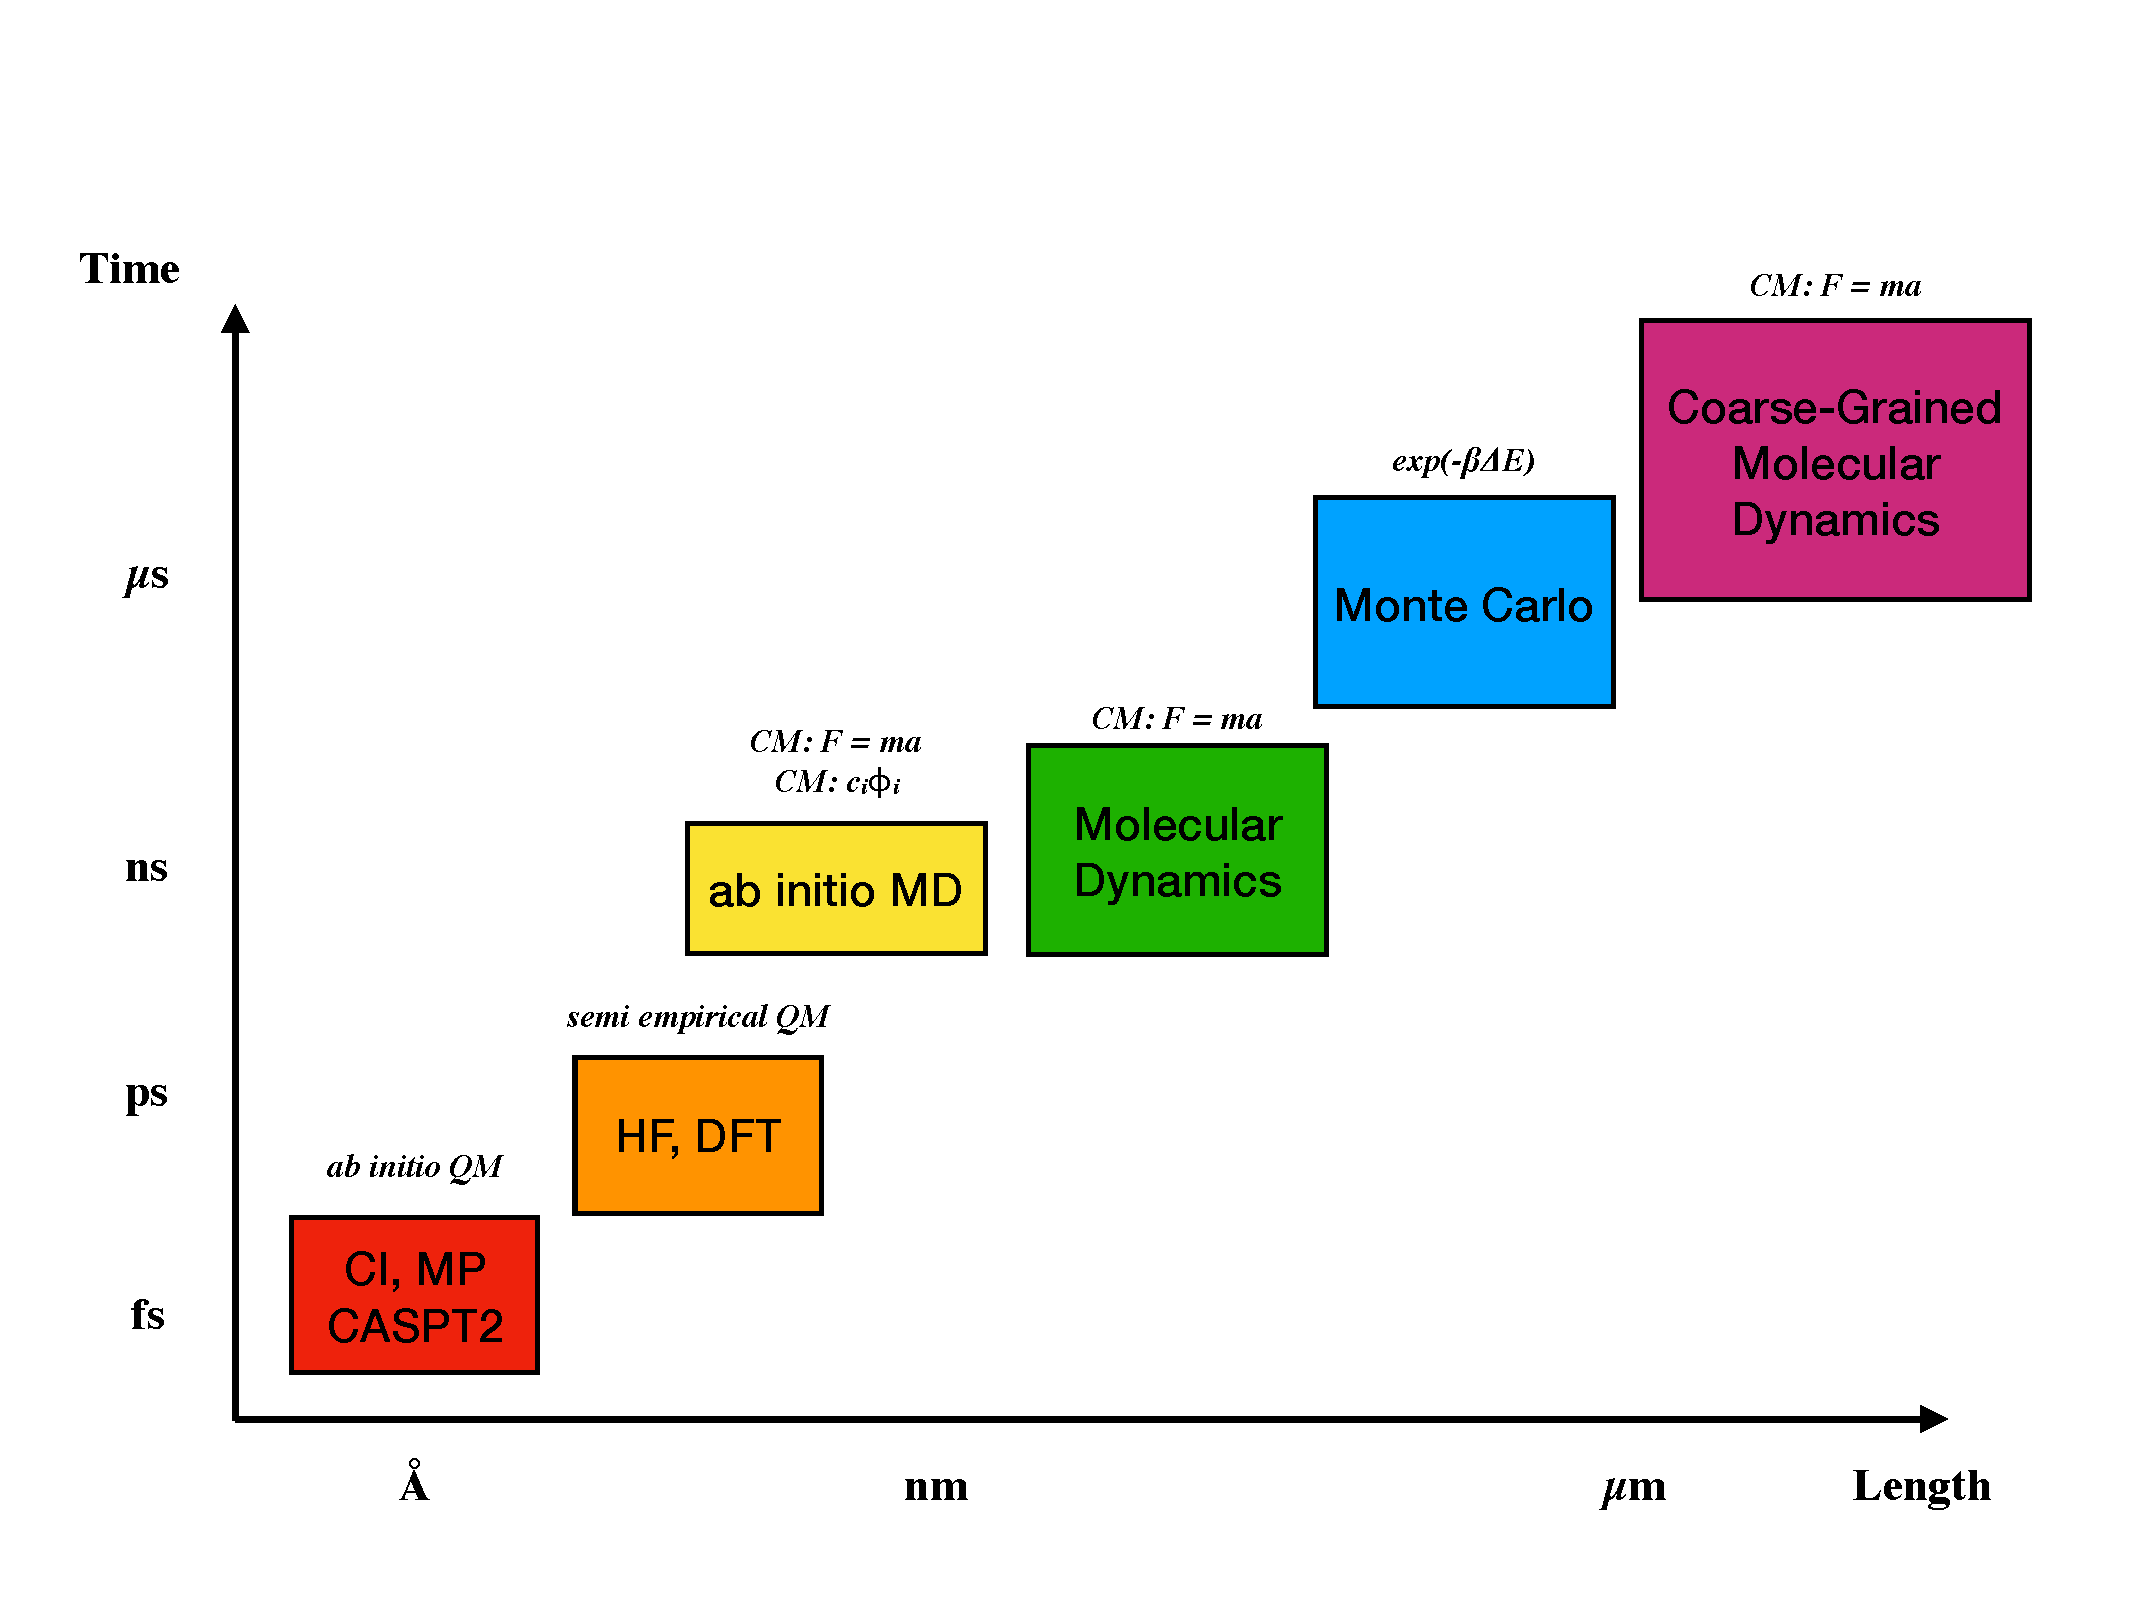
\includegraphics[width=\linewidth]{Figures/SimulationScale}
% \caption{\label{fig:SimulationScale} Different length scales in
%   numbers of molecules (here length of material) and corresponding
%   achievable simulation time for various molecular modeling
%   methodologies. High accuracy quantum mechanical methods (red and
%   orange) cannot simulate large numbers of molecules for long
%   times. Methods which reduce molecular detail and propagate by
%   classical mechanics (yellow and green) are able to achieve longer
%   simulation times for larger systems. Monte Carlo methods (blue)
%   remove the expense of computing dynamics altogether, and ultra
%   coarse-grained methods (violet) which approximate collections of
%   atoms as a single unit achieve even longer simulation times.}
% \end{figure}
In 1812, Pierre Simon Laplace published a manuscript entitled
\textit{A Philosophical Essay on Probabilities} detailing his system
of reasoning based on probabilities.\cite{Laplace1902} Within this
work, he describes the notion of casual or scientific determinism,
that is, that all events are dictated by previously existing causes:
 
\begin{displayquote}
We may regard the present state of the universe as the effect of
its past and the cause of its future. An intellect which at a certain
moment would know all forces that set nature in motion, and all
positions of all items of which nature is composed, if this intellect
were also vast enough to submit these data to analysis, it would
embrace in a single formula the movements of the greatest bodies of
the universe and those of the tiniest atom; for such an intellect
nothing would be uncertain and the future just like the past would be
present before its eyes.
\end{displayquote}

This became known as Laplace's Demon, and a desire to confirm or
refute this claim was a significant driving force in the development
of statistical thermodynamics.  At the beginning of the 19th century,
concepts of irreversibility, entropy, and the second law of
thermodynamics suggested Laplace's Demon as being inaccurate.
Stochastic models for chaos theory and quantum mechanics provided
additional evidence against the claim, and it now agreed upon as
untrue.

Still, today we strive to achieve the premise that Laplace founded,
relinquishing the unobtainable absolute predictability of nature for
solvable representative models, stepping slowly towards understanding
the universe. We have replaced the `powerful intellect' with
computers, and develop algorithms to iteratively solve these
complex models. Through computer simulations we are becoming more
proficient at understanding and predicting the world around us, from
the motion of planets to the properties of molecules.

\section{Molecular Dynamics}
In general, molecular dynamics (MD) simulations involve propagating
the coordinates of numerical models of molecules through time using
Newton's Second Law. The models used to describe the molecules are
often constructed using classical mechanics, treating atoms as hard
spheres and bonds between atoms in a molecule as a spring. Charges are
also handled classically, and depending on the model the charges can
be static (restricted to some initial value), or dynamic, in which
they allowed to fluctuate in response to an external field. While
hybrid quantum / classical molecular dynamics methods exist, we
restrict ourselves here to the purely classical case. In the following
sections, I outline the basis of classical molecular dynamics
simulations. References for what is presented here comes from several
excellent books which cover molecular dynamics, from the classic text
of Allen and Tildesey, to the work of
Leach.\cite{Allen1987,Leach2001}

We begin by considering a many-body expansion of the configurational
potential energy $\mathscr{U}$ for an isolated collection of $N$ particles with
vector coordinates $\mathbf{r}^N$.
\begin{equation}\label{eq:potE}
  \mathscr{U}(\mathbf{r}^N) = \sum_i U(\mathbf{r}_i) + \sum_{i<j}
  U(\mathbf{r}_i,\mathbf{r}_j) + \sum_{i<j<k}
  U(\mathbf{r}_i,\mathbf{r}_j,\mathbf{r}_k) + \dots + U(\mathbf{r}_1,\mathbf{r}_2,\mathbf{r}_3,\dots \mathbf{r}_N)
\end{equation}
Most commonly, the expansion is truncated at the two-body term as
higher order terms have proven too computationally expensive
. However, with the development of faster computers, Paesani
\textit{et al.} has recently shown that incorporating higher order
terms leads to a more accurate water model.\cite{Paesani2016} A more
detailed discussion on water models will be presented in Section
\ref{sec:WaterModels}; for now, we will restrict ourselves to a
many-body expansion up to the two-body term. We further restrict
ourselves to a potential where no dissipative forces act between
particles, from this, we can obtain the force on particle $i$.
\begin{equation}\label{eq:force}
\mathbf{F_i} = -\frac{\partial \mathscr{U}(\mathbf{r}^N)}{\partial \mathbf{r}_i}
\end{equation} 
Since the system of $N$ particles is isolated and there are no
dissipative forces, the total energy of the system will be
conserved. From Equation \eqref{eq:force} and Newton's Second Law, the
accelerations for each of the $N$ particles follows,
\begin{equation}\label{eq:accel}
 m_i\mathbf{\ddot{r}}_i = -\frac{\partial \mathscr{U}(\mathbf{r}^N)}{\partial \mathbf{r}_i}
\end{equation}
Integrating Equation \eqref{eq:accel} once with respect to time gives
the momenta of the $N$ particles, and a second integration gives the
positions.

\subsection{Finite Difference Methods and Equations of Motion}
For particles described by a continuous potential energy function, the
forces acting upon each of the $N$ particles will change every time
the particles moves. Therefore, the motions of all particles are
coupled, giving rise to a many-body problem with no analytic
solution. Therefore, finite difference methods of integration must be
used in order to propagate the coordinates of the particles through
time.

While there exist a large number of algorithms for propagating
coordinates, they are not all equivalent. The general idea for each
method is to take small steps through time ($\delta t$) by knowing the
position and momenta for each of the $N$ particles at a previous time
($t-\delta t$). Knowing these quantities, the forces are calculated
from the position at time $t$, and the positions and momenta are
updated accordingly. This results in a new $\mathbf{r}^N$
configuration, and the method iterates again.

The main difference between integration schemes is what data is stored
between steps. In the \textit{Verlet} method, two sets of positions
are stored as well as a single set of accelerations. The velocity
terms do not appear explicitly but can be computed from the two sets
of positions. In the \textit{Leap Frog} method, the positions and
velocities are stored at half-steps. When the positions are known at a
half-step forward in time, the new velocities are computed and
`leap-frog' over the positions. While this method is an improvement
over the Verlet algorithm as the velocities are computed directly, the
positions and velocities are not known at the same time without
further calculation.

In our work, the \textit{velocity Verlet} method was used. In this
integration scheme the positions, velocities, and accelerations are
known at the same time. Given an initial set of positions at time $t$,
the accelerations, $\mathbf{\ddot{r}}(t)$, can be computed from
Equation \eqref{eq:accel}. Together with the velocities at $t$, the
future values of these quantities can be determined.
\begin{equation}\label{eq:vv-r}
\mathbf{r}(t+\delta t) = \mathbf{r}(t) + \delta t \mathbf{\dot{r}}(t) +
\frac{1}{2}t^2\mathbf{\ddot{r}}(t)
\end{equation}
\begin{equation}\label{eq:vv-v}
\mathbf{\dot{r}}(t+ \delta t) = \mathbf{\dot{r}}(t) + \frac{1}{2}\delta
t[\mathbf{\ddot{r}}(t) + \mathbf{\ddot{r}}(t + \delta t)]
\end{equation}
This method has to be implemented in three steps, as the accelerations
at times $t$ and $t + \delta t$ must be known to update the
velocities. In the first step, the positions are updated to
$t + \delta t$ using the velocities and accelerations at time $t$. In
the second step, the velocities at time $t + \frac{1}{2} \delta t$ are
computed.
\begin{equation}\label{eq:vv-v2}
\mathbf{\dot{r}}(t+\frac{1}{2}\delta t) = \mathbf{\dot{r}}(t) + \frac{1}{2}\delta t
\mathbf{\ddot{r}}(t)
\end{equation}
Forces are computed using the new positions $\mathbf{r}(t + \delta
t)$, and from these forces the new accelerations $\mathbf{\ddot{r}}(t +
\delta t)$ are determined. Lastly the velocities at time $t + \delta
t$ are computed by
\begin{equation}\label{eq:vv-v3}
\mathbf{\dot{r}}(t+\delta t) = \mathbf{\dot{r}}(t+\frac{1}{2}\delta t) +
\frac{1}{2}\delta \mathbf{\ddot{r}}(t + \delta t)
\end{equation}


\subsection{Time Averages and Ensemble Averages}
Consider a property $A$ that is dependent on the positions and momenta
of the $N$ particles in the system, then the instantaneous value of
$A$ can be expressed as $A(\mathbf{r}^N(t),\mathbf{p}^N(t))$. As the
positions and momenta of the particles evolve, the value of $A$
fluctuates. During an experiment, a \textit{time average} of $A$ is
measured for a large collection of particles. As the duration of the
experiment increases, the value of the measured property approaches
the `true' value, $A_{\mathrm{ave}}$.
\begin{equation}\label{eq:A-ave}
A_{\mathrm{ave}} = \mathrm{lim}_{\tau \to \infty} \frac{1}{\tau} \int_{t=0}^{\tau}
A(\mathbf{r}^N(t),\mathbf{p}^N(t))\mathrm{d}t
\end{equation}

In theory, it is straightforward to compute the time averaged value of
$A$ from a computer simulation. As described previously, the positions
and velocities can be integrated through time, and for each
configuration of the system $A(\mathbf{r}^N(t),\mathbf{p}^N(t))$ could
be computed. The issue arises when considering a macroscopic number of
particles ($10^{23}$), as calculation of even the initial time step is
infeasible. Instead, we turn to statistical mechanics as a connection
between a microscopic system ($10^2 - 10^6$ particles) and the
macroscopic experimental observation. Here, instead of considering one
large system, we evolve a large number of replicas of a smaller
system simultaneously. The average value of the property from these
replicas is defined as an \textit{ensemble average}, and is denoted
with angle bars, $\langle$~ $\rangle$.
\begin{equation}\label{eq:A-ens}
\langle A \rangle = \int \int \mathrm{d}\mathbf{r}^N \mathrm{d}\mathbf{p}^N
A(\mathbf{r}^N,\mathbf{p}^N) \rho
(\mathbf{r}^N,\mathbf{p}^N)
\end{equation}
Equation \eqref{eq:A-ens} is written as a double integral, although
more accurately this equation indicates $6N$ integrals, one for each
of the $3N$ position and $3N$ momentum coordinates of the $N$
particles. The second factor in the integrand,
$ \rho(\mathbf{r}^N,\mathbf{p}^N)$, is the \textit{probability
  density} of the ensemble. It is a function which describes the
relative probability of observing a specific configuration and
distribution of momenta for the $N$ particles, given the energy of the
configuration. If one is able to compute $\langle A \rangle$ by
integrating over all possible configurations of the system, the
resulting ensemble average will be equal to the time average value
($A_{\mathrm{ave}} = \langle A \rangle$) by the \textit{ergodic
  hypothesis}. In practice, it is not often possible to integrate over
all possible configurations. Instead, convergence of the property
$\langle A \rangle$ is achieved once the system has explored a
sufficient amount of phase space.

\subsection{Calculation of Thermodynamic Properties}
As the particles evolve through time, there are several possible
thermodynamic properties which we may wish to compute. Among the
properties most commonly desired are the temperature and pressure.
The instantaneous temperature, $T$, of a collection of $N$ molecules
is related to the kinetic energy through the equipartition
theorem.
\begin{equation}\label{Temperature}
T = \frac{2}{fk_B}\Bigg( \sum_{i=1}^{N} \frac{1}{2} m_i {\bf v}_i^T \cdot {\bf v}_i +
\sum_{i=1}^{N_{\mathrm{linear}}+N_{\mathrm{non-linear}}}  \frac{1}{2} {\bf j}_i^T \cdot
\overleftrightarrow{\mathsf{I}}_i^{-1} \cdot {\bf j}_i  \Bigg)
\end{equation}

where $f$ is the total number of degrees of freedom in the system,
\begin{equation}
f = 3 N + 2 N_{\mathrm{linear}} + 3 N_{\mathrm{non-linear}} - N_{\mathrm{constraints}}
\end{equation}
$k_B$ is Boltzmann's constant, $N_{linear}$ is the number of linear
rigid bodies, and $N_{non-linear}$ is the total number of non-linear
rigid bodies in the system. The first sum includes the linear velocities
of all $N$ bodies, while the second sum is over those with angular
velocity $\bf j_i$, and moment of inertia,
$\overleftrightarrow{\mathsf{I}}_i$.

The instantaneous pressure, $P$, of a collection of particles can be
obtained through the virial theorem of Clausius. The \textit{virial},
$W$, is defined by
\begin{equation}\label{eq:virial}
W = \sum_{i=1}^N \sum_{\alpha=1}^n r_{i\alpha}\dot{p}_{i\alpha}
\end{equation}
where $r_{i\alpha}$ is the position along the $\alpha$ axis for
particle $i$, and
$\dot{p}_{i\alpha}$ is the first time derivative of momentum, or force,
along that coordinate. The virial theorem of Clausius states that the
virial is equal to $-3Nk_BT$.

For an ideal gas, the molecules composing the gas only interact with
the walls of the container. Therefore, the only forces present in the
system are due to those between the gas and the container. In this
case, the virial becomes $-3PV$ directly from the ideal gas law. We
can consider a system of interacting particles as a perturbation from
the ideal gas case, where the virial for the interacting system would
be the ideal gas virial plus a contribution due to the interactions of
the particles.
\begin{equation}\label{eq:virial2}
W = -3PV + \sum_i^N \sum_{j\neq i}^N r_{ij} \frac{dU(r_{ij})}{dr_{ij}} = -fk_BT
\end{equation}
Here we have considered a potential consisting of only two-body
interactions, although expansion to higher-order terms is
straightforward. If we instead write Equation \eqref{eq:virial2} in terms
of the force between particles $i$ and $j$, ($f_{ij}$), we obtain the
following expression for the pressure.
\begin{equation}\label{eq:virial3}
P = \frac{1}{V}\Big[fk_BT - \frac{1}{3} \sum_i^N \sum_{j\neq i}^N
r_{ij} f_{ij}\Big]
\end{equation}

These are just two of many thermodynamic properties one may wish to
compute as a simulation evolves. The problem of writing expressions
for the desired properties in terms of particle positions and
velocities lies at the heart of the matter. Once established, solving
the equations at regular intervals of simulation time becomes
straightforward. As an interesting final remark on this section, we
note that while two identical collections of particles (with the exact
same set of positions and velocities) evolving under different
potential energy functions will reproduce the same temperature for
that configuration, the associated pressures (and many other
thermodynamic properties) will be different. Therefore, we should
expect collections of the same molecules (\textit{e.g.} water)
described under different potential energy functions or parameters, to
result in vastly different thermodynamic properties.

\subsection{Molecular Force Fields}
Having established how to propagate particles through time using MD
simulations, we turn our focus next to the problem of developing an
accurate representation for the interactions between molecules, more
commonly known as a force field. Generally, the functional form of the
force field is structured as a balance between accurately capturing
the pertinent physics and what is feasible given computational
resources. Here, we present functional forms for force fields commonly
used, followed by a discussion of suitable parameters in a brief
overview of the large body of literature surrounding water models.

Due to computational expense, it is common to truncate the many-body
expansion of the potential energy to include only the one-body and
two-body interaction terms, and consider only those two-body terms
which are pairwise additive. That is, the potential in Equation
\eqref{eq:potE} becomes,
\begin{equation}\label{eq:potPair}
\mathscr{U}(\mathbf{r}^N) = \sum_i^N U(\mathbf{r}_i) + \sum_{i<j}^N U(r_{ij})
\end{equation}
where $\mathbf{r}_i$ is the absolute position of particle $i$, and
$r_{ij}$ is the scalar distance between particles $i$ and $j$,
$r_{ij} = | \mathbf{r}_j - \mathbf{r}_i|$. This may seem like an
extreme restriction on the potential, however, we will see models with
this structure still perform quite well.

The one-body term in Equation \eqref{eq:potPair} accounts for any
external forces on the particles, such as an electric field. Their
interaction with the field depends on the particle's absolute position
in that field, not the relative distance between it and the other
particles. In the absence of an external potential, Equation
\eqref{eq:potPair} reduces to just the two-body pairwise additive
term, and the potential only depends upon the relative distance
between particles. Generally, these terms fall into one of two
categories, bonded and non-bonded interactions.

\subsubsection{Bonded Interactions}
There are three bonded terms (often referred to as short-ranged
interactions) which deserve discussion. Bonds between two atoms in a
molecule, bends between two atoms centrally connected to a third, and
torsions between four consecutively bonded atoms. Bonds are often
treated as harmonic oscillators, with a spring constant $k_{ij}$ set
to mimic the stiffness of the bond and equilibrium distance set to the
bond length $r_{ij}^0$. The spring constant is determined from the
frequency of the bond $\omega$ and the reduced mass $\mu_{ij}$ of the
two atoms in the bond.
\begin{equation}
\mu_{ij} = \frac{m_i m_j}{m_i + m_j}
\end{equation}
\begin{equation}\label{eq:kij}
\omega = \sqrt{\frac{k_{ij}}{\mu_{ij}} }
\end{equation}

\begin{equation}\label{eq:bonds}
U_{bond}(r_{ij}) = \frac{1}{2} k_{ij} (r_{ij} -r_{ij}^0)^2
\end{equation}

Similarly, bends within a molecule are also treated as harmonic
oscillators, with spring constants $k_{\theta_{ijk}}$ and equilibrium bend
angles $\theta_{ijk}^0$. However, while the bonding potential is a
function of the distance between particles $i$ and $j$, the bending
potential is more succinctly written as a function of the angle formed between three
consecutively bonded atoms $i$, $j$, and $k$,
\begin{equation}\label{eq:bend}
\theta_{ijk} = \mathrm{cos}^{-1}\Bigg(\frac{\mathbf{r}_{ji} \cdot
  \mathbf{r}_{jk}}{|r_{ji}|~|r_{jk}|}\Bigg)
\end{equation}
where atom $j$ is the central atom. 
\begin{equation}\label{eq:bend2}
U_{bend}(\theta_{ijk}) = \frac{1}{2} k_{\theta_{ijk}} (\theta_{ijk} -
\theta_{ijk}^0)^2
\end{equation}

A torsion describes a rotation of groups about a central bond, and is
often expressed in terms of a cosine expansion.
\begin{equation}\label{eq:torsion}
U_{torsion}(\phi_{ijkl}) = c_1[1+\mathrm{cos}\phi_{ijkl}] + c_2[1-\mathrm{cos}(2\phi_{ijkl})]+c_3[1+\mathrm{cos}(3\phi_{ijkl})]
\end{equation}
Here, the angle $\phi_{ijkl}$ is defined as
\begin{equation}\label{eq:torsion2}
\mathrm{cos}\phi_{ijkl} = \frac{(\mathbf{\hat{r}}_{ij} \times
\mathbf{\hat{r}}_{jk}) \cdot (\mathbf{\hat{r}}_{jk} \times
\mathbf{\hat{r}}_{kl})}{|\mathbf{\hat{r}}_{ij} \times
\mathbf{\hat{r}}_{jk}|~|\mathbf{\hat{r}}_{jk} \times
\mathbf{\hat{r}}_{kl}|}
\end{equation}
and the coefficients $c_1$, $c_2$, and $c_3$ are terms describing the
barrier for transitioning from a \textit{cis} to a \textit{trans}, or \textit{staggered} to
\textit{eclipsed} conformations.

\subsubsection{Non-bonded Interactions}
In 1903, Gustav Mie proposed a pairwise additive
non-bonded potential for a system of soft-spheres.
\begin{equation}\label{eq:LJ}
U_{\mathrm{Mie}}(r_{ij}) = k\epsilon_{ij}\Bigg[ \Big( \frac{\sigma_{ij}}{r_{ij}}\Big)^n - \Big(\frac{\sigma_{ij}}{r_{ij}}\Big)^m\Bigg]
\end{equation}
where
\begin{equation}\label{eq:LJ2}
k = \frac{n}{n-m} \Big(\frac{n}{m}\Big)^{m/(n-m)}.
\end{equation}
With this simple model, Mie was able to account for both short-ranged
repulsive forces as well as long-range attractive forces. The
short-ranged forces are important to keep a collection of particles
from collapsing in on itself, while the long-range forces prevents the
collection of particles disintegrating. In 1924, J. E. Lennard-Jones
proposed a specific form of the Mie potential for molecular
simulation. Since the leading term in London's theory on dispersion
forces goes at $1/r^6$, the long-range term is chosen to mimic this
behavior $m=6$. While there is no physical justification for it, the
short-ranged attraction term is often set to $n=12$ primarily due to
ease of computation. With these values for $m$ and $n$ the resulting
Lennard-Jones model becomes
\begin{equation}\label{eq:LJ3}
U_{\mathrm{LJ}}(r_{ij}) =
4\epsilon_{ij}\Bigg[\Big(\frac{\sigma_{ij}}{r_{ij}}\Big)^{12}-\Big(\frac{\sigma_{ij}}{r_{ij}}\Big)^{6}\Bigg].
\end{equation} 
The remaining two parameters to the model are $\sigma_{ij}$, the distance
at which $U_{\mathrm{LJ}}(r_{ij})$ goes to zero, and $\epsilon_{ij}$, the potential
energy minimum which is located at $r_{ij} = \sqrt[6]{2}\sigma_{ij}$. While the
number and locations of Lennard-Jones sites within water models vary,
the parameter $\sigma$ is commonly taken to be the molecular diameter
and $\epsilon$ is often tuned to reproduce a certain region of the
phase diagram. Interactions between different types of particles
requires a mixing of the parameters $\sigma$ and $\epsilon$. These are
normally determined by the Lorentz-Berthelot mixing rules, where
$\sigma_{ij}$ is determined by an algebraic mean 
\begin{equation}\label{eq:sigma}
\sigma_{ij} = \frac{1}{2} [\sigma_{ii} + \sigma_{jj}]
\end{equation}
and $\epsilon_{ij}$ is taken as the geometric mean of $\epsilon$ for
particles $i$ and $j$. \cite{Lorentz1881,Berthelot1898}
\begin{equation}\label{eq:epsilon}
\epsilon_{ij} = \sqrt{\epsilon_{ii}\epsilon_{jj}}
\end{equation}


A second non-bonded interaction we must consider is the appropriate
treatment of charged particles. Commonly, molecular mechanics
forcefields represent molecular charges as point charges on atomic
sites, coupled with short-ranged Lennard-Jones repulsions to prevent
molecules from collapsing onto one another. While there are many
methods for computing these interactions, Coulomb's law is
at the heart of the methods.
\begin{equation}\label{eq:coulomb}
U_{\mathrm{charge}}(r_{ij}) = \sum_{ij}\frac{q_i q_j e^2}{4 \pi \epsilon_0
  r_{ij}}
\end{equation}
Here, $q_i$ and $q_j$ are the charges on particles $i$ and $j$, $e$ is
the charge of an electron, and $\epsilon_0$ is the permittivity of
free space. 

For a system of $N$ molecules, the number of bonded terms goes as $N$
but the number non-bonded interactions as $N^2$.  Computing the
non-bonded interactions is therefore the most computationally expensive
part of the simulation. The Lennard-Jones interaction, however, falls
off quite rapidly due to its $r^{-6}$ functional form. Meanwhile, the
long-ranged $r^{-1}$ decay of electrostatic interactions can have
significant value at distances as large as the simulation cell. These
interactions are quite problematic and will be addressed in the
following paragraphs. However, we will first discuss adding a cutoff
to the potential, a method commonly used to save computation time.

% Make cutoff small enough that particle doesn't see its own
% image. Neighbor-lists make cutoffs worthwhile, otherwise we would have
% to compute all pairwise distance each timestep to determine if we
% should compute potential and forces or not. In larger systems, a cell
% index method can be used where the molecules are cast into mini cells,
% and then neighbor lists are constructed from the 26 cells surrounding
% the cell in question (total of 27 cells then). Sorting molecules is on
% order $N$, and sorting neighbors is cheap as long as the total number
% of cells is greater than 27.

When using a cutoff radius, the potential is evaluated unmodified for
distances less than the cutoff, and set to zero for objects outside
the cutoff. This introduces discontinuities in the potential and thus
the force calculations. One way to prevent potential discontinuities
is to shift the potential by its value at the cutoff.  The additive
constant vanishes upon taking the derivative to compute the forces,
and energy conservation is better than with the unshifted
potential. However, there is still a problem of  discontinuities in the
forces with this method. A second solution is to use a switching
function to smoothly transition the potential to zero at the cutoff.

% Switching functions can take several forms, one
% such example is the following polynomial
% \begin{equation}
% v'(r) = v(r)\Big[1-2\Big(\frac{r}{r_c}\Big)^2 + 
% 4\Big(\frac{r}{r_c}\Big)^4 \Big]
% \end{equation}
% The switching function has a value of $1$ at $r=0$ and $0$ at
% $r = r_c$. Switching functions are normally implemented at some
% distance close to the cutoff, so that only a small amount of the
% potential is perturbed. This prevents aspires affects such as
% deviation from equilibrium structures. Need the first derivative of
% the switching function at the end points to be zero to ensure the
% forces approach zero smoothly, and second derivatives to be zero for
% stability of integration algorithm. 
% \begin{equation}
% S(r) = c_0 + c_1\Big[\frac{r-r_l}{r_u-r_l}\Big] +
% c_2\Big[\frac{r-r_l}{r_u - r_l}\Big]^2
% + c_3\Big[\frac{r-r_l}{r_u-r_l}\Big]^3 +
% c_4\Big[\frac{r-r_l}{r_u-r_l}\Big]^4 +
% c_5\Big[\frac{r-r_l}{r_u-r_l}\Big]^5
% \end{equation}
% The set of coefficients that satisfies the derivative stipulations are
% $(c_0 = 1, c_1 = 0, c_2 = 0, c_3 = -10, c_4 = 15, c_5 = -6)$.

Interactions that decay no faster than $r^{-n}$ where $n$ is the
dimensionality of the system can pose a problem in that they may not
converge for distances greater than the size of the simulation
box. Charge-charge interactions go as $r^{-1}$, and therefore are
quite problematic. There have been several methods suggested to handle
this issue, the most famous of which is the method presented by Ewald
in 1921. The Ewald Sum requires replicas of the simulation cell for
computation of $U_{charge}(r_{ij})$. These charges are wrapped by
a Gaussian of opposite charge, creating a screen around the
charges. Doing so requires two corrections to be made; first, an
oppositely charged Gaussian must also be added for each one introduced
around a charge. Secondly, since the Gaussians interact with
themselves, a self correction piece must be added. Depending
on the material being modeled, a dipole correction might also need to
be added. The charges and the Gaussians screening them are added
up in real space, while the oppositely charged Gaussians are added in
reciprocal space. This method is computationally very expensive.
However, it is the most accurate way of computing the charge-charge
interactions in molecular simulation. 

An alternative approach to the demanding Ewald Sum is the method first
developed by Wolf \textit{et al.}\cite{Wolf1999}, and later expanded
upon by Fennel and Gezelter.\cite{Fennell2006} This method combines
shifting the potential as described above with a dampening of the
electrostatic interactions in a similar fashion as the Ewald
Summation. The first key observation is that the electrostatic
interactions are shorter ranged than $r^{-1}$ in condensed
phases. Wolf \textit{et al.}  observed that creating a neutral cutoff
sphere resulted in a good conservation of energy. Fennell and Gezelter
began with the standard shifted potential,

\begin{equation}
V_\textrm{SP}(r) =      \begin{cases}
v(r)-v_\textrm{c} &\quad r\leqslant R_\textrm{c} \\ 0 &\quad r >
R_\textrm{c}  
\end{cases},
\label{eq:shiftingPotForm}
\end{equation}
and expanded on this to arrive at the shifted force,
\begin{equation}
V_\textrm{SF}(r) =      \begin{cases}
v(r)-v_\textrm{c}-\left(\frac{d v(r)}{d r}\right)_{r=R_\textrm{c}}(r-R_\textrm{c
})
&\quad r\leqslant R_\textrm{c} \\ 0 &\quad r > R_\textrm{c} 
                                                \end{cases},
\label{eq:shiftingForm}
\end{equation}

which guaranteed the potential and forces smoothly go to zero at the
cutoff radius, $R_\textrm{c}$. Wolf \textit{et al.} observed that when
the potential is taken to be the Coulomb potential, Equation
\ref{eq:coulomb}, the calculated Madelung energies fluctuated around
the analytic value with increasing size of the cutoff radius, with a
slow decay towards the expected value.\cite{Wolf1999} Therefore, to
accelerate the convergence of the expected energies, a dampening
function was introduced resembling the effective screening of the
oppositely charged Gaussians in the Ewald summation. Doing so, Fennell
and Gezelter arrived at the following damped shifted force,

\begin{equation}
\begin{split}
V_\mathrm{DSF}(r) = q_iq_j\Biggr{[} & \frac{\mathrm{erfc}\left(\alpha r \right)}{r} -\frac{\mathrm{erfc}\left(\alpha R_\mathrm{c} \right) }{R_\mathrm{c}} \\
 & \left. +\left(\frac{\mathrm{erfc}\left(\alpha
R_\mathrm{c}\right)}{R_\mathrm{c}^2}+\frac{2\alpha}{\pi^{1/2}}\frac{\exp\left(-\alpha^2R_\mathrm{c}^2\right)}{R_\mathrm{c}}\right)\left(r-R_\mathrm{c}\right)
\right] \quad r\leqslant R_\textrm{c} 
\label{eq:DSFPot}
\end{split}
\end{equation}
where $\mathrm{erfc}$ is the complimentary error function with dampening
parameter $\alpha$. Taking the derivative of this damped shifted force
potential will lead to the following expression for forces,
\begin{equation}
\begin{split}
F_\mathrm{DSF}(r) =
q_iq_j\Biggr{[}&\left(\frac{\textrm{erfc}\left(\alpha r\right)}{r^2}+\frac{2\alpha}{\pi^{1/2}}\frac{\exp{\left(-\alpha^2r^2\right)}}{r}\right) \\ &\left.-\left(\frac{\textrm{erfc}\left(\alpha R_{\textrm{c}}\right)}{R_{\textrm{c}}^2}+\frac{2\alpha}{\pi^{1/2}}\frac{\exp{\left(-\alpha^2R_{\textrm{c}}^2
\right)}}{R_{\textrm{c}}}\right)\right] \quad r\leqslant R_\textrm{c}.
\label{eq:DSFForces}
\end{split}
\end{equation}
Fennell and Gezelter have shown that the damped shifted force method
gives nearly identical results when compared with the smooth particle
mesh Ewald method on a variety of commonly simulated
systems.\cite{Fennell2006}

\subsection{Boundary Conditions}
Having discussed how to evolve particle positions and momenta through
time under a classical potential, we now focus on the problem of how
to simulate a tractable number of particles. Consider an open (but
isolated) system of particles. The cluster would be exposed to vacuum
in all three dimensions, and depending on the strength of the
intermolecular interactions, the cluster could condense into a sphere
or slowly dissipate into a gas. If we were interested in simulating a
liquid, the vacuum exposed droplet would be a poor representation of a
bulk fluid.

A naive approach to fix this problem would be to simulate a large
cluster of molecules and only probe the properties of the interior
molecules. This is both inefficient and potentially inaccurate, as
determining when a cluster is `large enough' for the interior
molecules to recover bulk liquid behavior is open to
interpretation. An efficient solution to this problem is to impose
boundary conditions on the system. While the type of boundary
condition imposed can depend on the type of material being simulated,
cubic or parallelepiped periodic boundary conditions are the most
common. In these methods, the system of particles is
effectively replicated around the initial simulation cell. If a
particle leaves the simulation cell (\textit{e.g.} through the
positive $x$ dimension) then one of the images of the particle will
enter the cell through the opposite wall (from the negative $x$
dimension).

In Figure \ref{fig:PBC}, a two-dimensional representation of cubic
periodic boundary conditions shows how the true simulation cell (in
blue) has a constant number of particles (red circles). As a particle
leaves the initial cell an image of itself enters through one of the
ghost cells surrounding the box. This is achieved by either wrapping
the position of each particle back to the initial cell after each
timestep, or by computing the potential energy and force calculations
using the ghost images. Notice that the nearest particles within the
cutoff radii, $r_{\mathrm{cut}}$, may be an image of a particle in one
of the ghost cells. Using this method, it is possible to simulate a
bulk fluid (or more generally a bulk material) using a tractable
number of particles.

\begin{figure*}
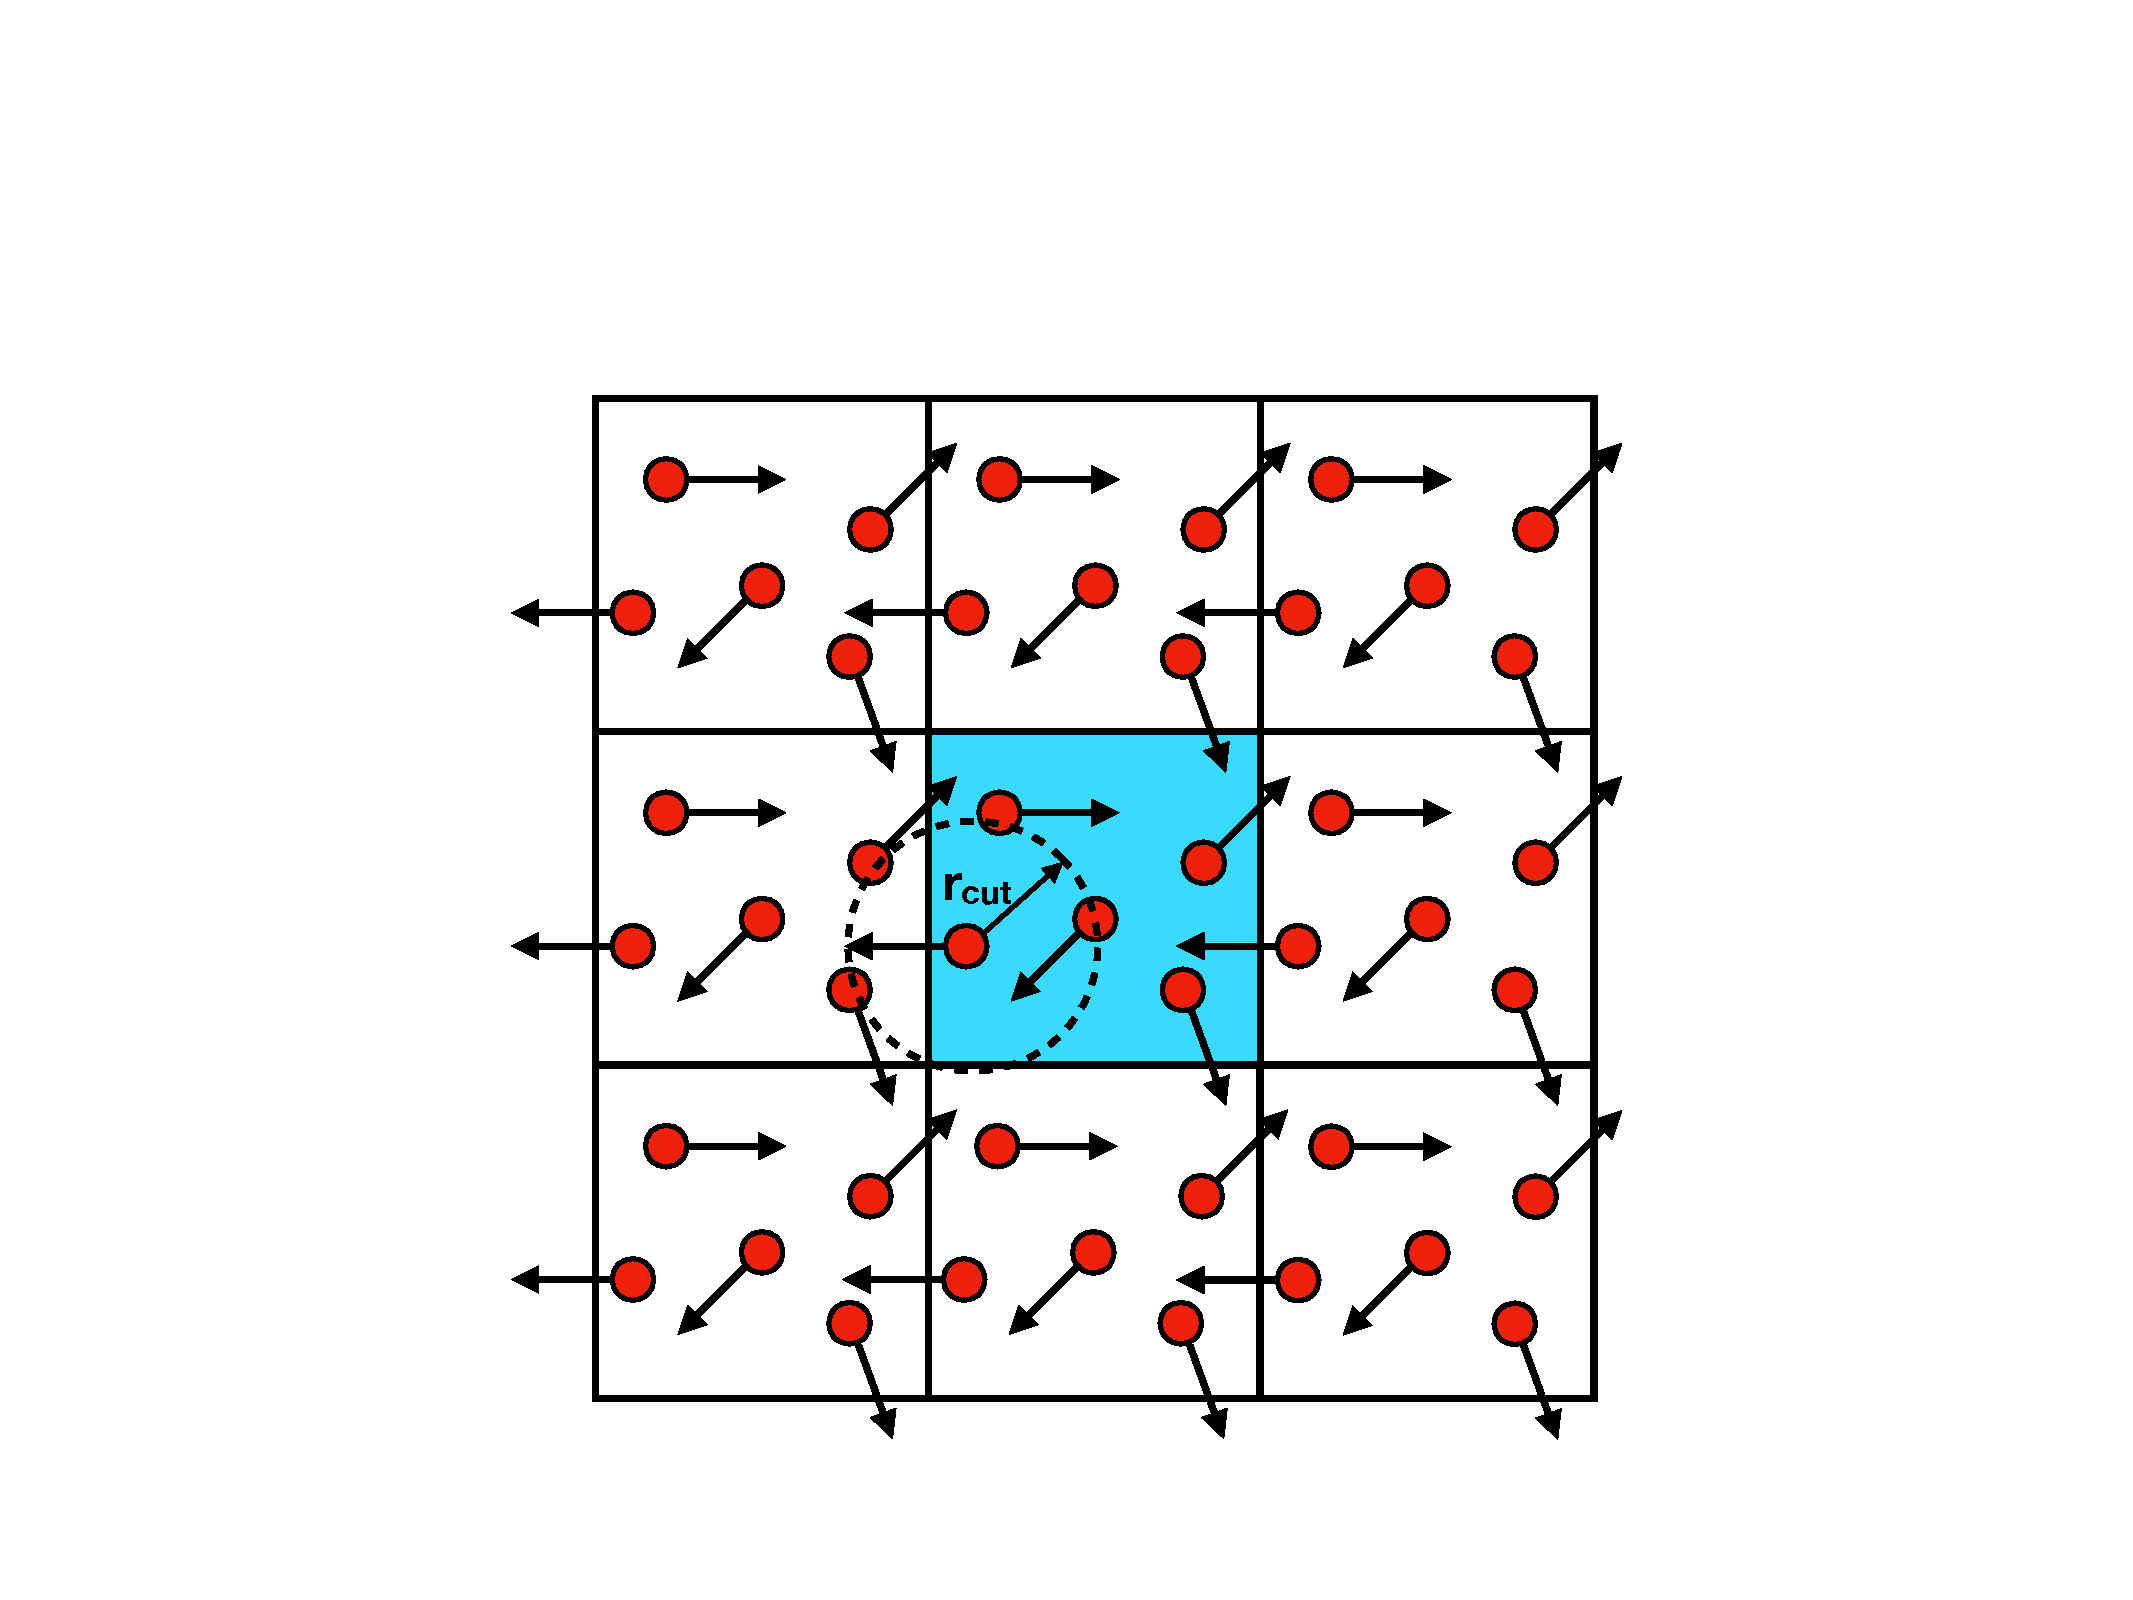
\includegraphics[width=\linewidth]{Figures/PBC}
\caption{\label{fig:PBC} Periodic boundary conditions and minimum
  image calculation. The central blue cell is the only simulation cell
  maintained by computation. Molecules (red circles) are free to move
  throughout space unhindered. When a molecule leaves the blue
  simulation cell, one of its ghost images enters the cell from one of
  the neighboring cells. This is achieved by computation of
  interactions of a molecule with its nearest neighbors within a
  cutoff radius of $r_{\mathrm{cut}}$. Note these molecules may not
  necessarily be located within the same simulation cell as the
  molecule of interest.}
\end{figure*}

Utilizing periodic boundary conditions does pose one potential
problem. If the unit cell length is not large compared to
$r_{\mathrm{cut}}$, then there is the possibility that a particle
could interact with an image of itself. Also, these methodologies
capture short wavelength events quite well, but it is impossible to
observe a phenomena with fluctuations or wavelengths larger than the
unit cell dimensions. This includes events near liquid-gas critical
points, and some phase transitions. However, unnecessarily large unit
cells require an increasing number of particles in the simulation, and
resulting computational times are often intractable.



\subsection{Water Models}\label{sec:WaterModels}
An investigation of the properties and dynamics of water anywhere in
the phase diagram cannot be conducted without first critically
analyzing the model proposed for the study. After almost 50 years of
simulating water, we are still optimizing and searching for geometries
and distributions of charges, potential sites, mass sites, and many
other parameters which will reproduce the phase diagram of water in
better agreement with experiments. However, in this time we have
learned much about the rich behavior and characteristics of water
through molecular simulations.

In this section we present a short review over the large body of
literature surrounding water models for molecular simulations. The
list of water models presented here is by no means complete, nor is
the analysis of these models exhaustive. There are a number of
excellent reviews on these topics, from the early reviews of
Brodsky\cite{Brodsky1996}, Wallqvist and Mountain\cite{Wallqvist1999},
Finney\cite{Finney2001}, and Guillot\cite{Guillot2002}, to the more
recent works of Ouyang\cite{Ouyang2015}, Cisneros\cite{Cisneros2016},
Gallo\cite{Gallo2016}, and Brini\cite{Brini2017}. We would be remiss
if we also did not include the significant contributions from Vega,
Abascal, Conde, Sanz, and
MacDowell.\cite{MacDowell2004,Vega2005,Vega2005c,Abascal2007,Abascal2007a,Abascal2007b,Abascal2007c,Vega2009,Vega2011,Vega2011a,Vega2015}
Lastly, we must acknowledge the expansive catalog of literature on
water by Martin Chaplin.\cite{Chaplin2018}

The first simulations of water were performed in 1969 by Barker and
Watts,\cite{Barker1969} and shortly thereafter by Rahman and
Stillinger in 1971\cite{Rahman1971} using the Ben-Naim Stillinger
potential\cite{Ben-Naim1972}. These inaugural investigations used
rigid, non-polarizable models for water, consisting of Lennard-Jones
and charge sites describing the intermolecular interactions, evolving
according to classical mechanics. Soon thereafter, Rahman and
Stilleger proposed the five-site ST2 model, which better captured the
density maximum for liquid water, and whose distribution functions
more accurately matched x-ray scattering data.\cite{Stillinger1974}

Since this time, hundreds of water models have been proposed and
characterized.\cite{Chaplin2018} These range from computationally
expensive models such as the SWM-4DP\cite{Lamourex2003},
TIP4P-FQ\cite{Rick1994}, DPP2\cite{Kumar2010},
TTM3-F\cite{Fanourgakis2008}, and AMOEBA\cite{Ren2003,Ren2004} models
which have moved beyond point charges and the pairwise additive
approximation and allow for anisotropic multipole polarizations, while
others have attempted to make large scale simulations more feasible by
collapsing the water molecule onto a single interaction
site\cite{Liu1996,Tan2003,Fennell2004}.

\subsubsection{Classes of Water Models}
Most commonly, water models are categorized by the number of
interaction sites and divided into subcategories by the types of
interactions described within the potential. Three, four, five, and
six site models are prevalent in the literature, although
computational expense increases with the number of interaction sites
($s$); as the number of non-bonded terms for $N$ molecules goes as
$s^N$. 

Here, we will focus on non-polarizable models, that is, models where
the charge distribution is held fixed and is not allowed to move
around the molecule. Similarly, we will restrict ourselves to rigid
models, where the OH bonds and HOH bends are held fixed in
space. While there are several models which propagate these degrees of
freedom, such as the SPC/f\cite{Ferguson1995}, SPC/Fw\cite{Wu2006},
and TIP4P/2005f\cite{Gonzalez2011} models, limiting our discussion to
models which exclude these degrees of freedom will provide a common
ground for comparison. 

The two most common three site models are Berendsen's
SPC/E\cite{Berendsen1987} and Jorgenson's TIP3P\cite{Jorgenson1983}
models. In both cases, the interaction sites are set to the atomic
positions, with positive charges on the two hydrogens and a negative
charge located on the oxygen. A Lennard-Jones interaction is also
defined on the oxygen site to prevent the molecules from collapsing
onto one another. The SPC/E model is a reparameterization of the
SPC\cite{Berendsen1981} model, where a self-energy correction was
included correcting the average polarization. With this correction,
the model more accurately reproduces the second neighbor peaks in the
pairwise radial distribution functions, as well as the density and the
diffusion at ambient conditions.\cite{Berendsen1987}

While attempting to determine the total internal energy of a water
molecule, Bernal and Fowler found that in order to reproduce the
observed dipole moment of water, they had to shift the negative charge
off of the oxygen towards the hydrogens along the HOH
bisector.\cite{Bernal1933} Following this idea, Jorgenson \textit{et
  al.} developed a four site water model, moving the negative charge
from the oxygen to a massless site along the HOH bisector. The
resulting TIP4P model more accurately reproduced oxygen-oxygen
diffraction data than the TIP3P model.\cite{Jorgenson1983} The four
site model was also found to have the correct density of liquid water
at ambient conditions. 

Due to the success of the TIP4P model, the four site structure has
been replicated and parameters refined spawning a large number of
models, including the TIP4P/Ew\cite{Horn2004},
TIP4P/2005\cite{Abascal2005a}, and TIP4P/Ice\cite{Abascal2005}
models. Simulations involving biomolecules often involve a large
number of charged species, as such, the TIP4P/Ew model is a
reparameterization of the TIP4P model for use with Ewald summation
methods. The TIP4P/2005 model was developed as a general purpose model
for condensed phases of water. Reparameterization was achieved using a
large amount of data from across the phase diagram. These data
include a fit of the temperature of maximum density, stability of
several ice polymorphs, the enthalpy of vaporization, and the density
of the liquid at ambient conditions. The resulting model gives good
agreement over a large span of the phase diagram, and has recently
been suggested as being the most accurate rigid non-polarizable model
to date.\cite{Vega2011a} 

In contrast to the parameterization of the TIP4P/2005 model where the
goal was to create a single model which spans much of the phase
diagram accurately, the TIP4P/Ice model was developed targeting the
properties of ice. The model was parameterized by fitting the equation
of state and selected points of the solid / liquid coexistence curves,
as well as several solid / solid coexistence curves for various ice
phases. The model gives excellent agreement for the melting
temperature of ice-I$_\mathrm{h}$, with T$_\mathrm{m} = $~272.2~K.

The category of five site models includes the ST2 model originally
proposed by Stillinger and Rahman in 1972\cite{Stillinger1974}, the
TIP5P model of Mahoney and Jorgensen\cite{Mahoney2000}, and its
reparameterization for use with Ewald summation methods (TIP5P/Ew) by
Rick.\cite{Rick2004} In the five site models, the negative charge has
moved out of the HOH plane, and is now distributed across two sites
mimicking electron lone pairs. The positive charges are located on
the hydrogen sites, and the Lennard-Jones position is placed on the
oxygen atom. The TIP5P model is observed to reproduce the density
maximum of water around 4\degree~C at 1~atm, and the dielectric
constant was found to be 81 $\pm$ 1.5 at 25\degree~C, in good
agreement with the experimentally known value (78.4). While these and
other properties predicted by the TIP5P model agree well with
experimental results, it has recently been shown that when one
considers performance of the model for a large number of properties,
the three site SPC/E and four site TIP4P/2005 water models outperform
the costly five site model. \cite{Vega2011a}

While six site models are rarely used, one is worth mentioning. The
NE6 model of Nada and van der Eerden is similar to the five site
models described above, with the addition of a massless charge site
along the HOH bisector.\cite{Nada2003a} This charge is taken to be
negative, however, the total molecule is constrained to be
neutral. The model was parameterized for simulations involving ice and
liquid near the melting point, and parameters were determined from
derivatives of the free energy of ice and water, as well as the
volumes of the same systems. Proton-disordered ice-I$_\mathrm{h}$ is
the stable structure at the melting point for the resulting NE6
model. The melting point was determined to be 271~$\pm$~9~K by Nada
and van der Eerden, in good agreement with the experimentally observed
273.15~K.

\subsubsection{Parameterizing Water Models}
After selecting the number of potential sites for a water model, the
next task is determining the interaction parameters associated with
each of those sites. Commonly, water models are parameterized in one
of two distinct ways, through \textit{ab initio} calculations or
matching empirical data. In the first method, high level quantum
mechanical calculations are performed on small clusters of water
molecules. From these, forces, stresses, and energies are obtained and
fit using a pairwise (or higher order) function to describe the
energy. In the second method, parameters for the interaction sites are
determined by iterative fitting against chosen experimental results,
such as the density or coexistence temperatures. A set of
interaction parameters are chosen, such as the charges ($\mathrm{q}_O$
and $\mathrm{q}_H$) and Lennard-Jones parameters ($\epsilon_O$ and
$\sigma_O$), and the resulting behavior of the water model is
recorded. The parameters are then iteratively changed until
convergence with the experimental data is achieved. 

Izadi and Onufriev have recently argued that the accuracy limit of the
rigid non-polarizable three and four site water models has been
achieved.\cite{Izadi2014,Izadi2016} In their initial work, they
iteratively solved for the optimal charge distribution for a four site
model.\cite{Izadi2014} The resulting OPC model reproduced bulk
properties more accurately than many other existing models. In
addition, the model also outperformed other models for predicting
hydration energies of small solute molecules. Following this, they
applied the same method for optimizing charge distributions to the
three site class of models. The resulting OPC3 model was observed
to reproduce liquid bulk properties better than other three site
models, such as the TIP3P and SPC/E models. The OPC3 model was also
found to accurately capture the intrinsic charge hydration asymmetry
of water. However, due to the complexity of the nature of water, these
models still perform poorly in extreme regions of the phase diagram,
\textit{i.e.} at regions far from where the models were parameterized.

\subsubsection{Melting Points of Common Water Models}
Ideally, the water model used to investigate the behavior of interest
will accurately reproduce the structure and dynamics of real water
around that region of the phase diagram. Assuming the model represents
real water accurately, inferences of the behavior of interest can then
be extracted from simulations. Therefore, the complete phase diagram
of water models are often characterized, in order to determine if it
is appropriate to use the proposed model for a given investigation.

Here, we are concerned with water near the solid / liquid and solid /
vapor coexistence regions. Therefore, it behooves us to critically
examine the reported melting points and coexistence lines of the
various ice polymorphs for water models of potential
interest. Recently, Vega, Garcia-Fernandez, Sanz, and Abascal have
computed and tabulated the melting points for many of the rigid
non-polarizable models discussed above, which we have reproduced in
Table
\ref{tab:meltingPoints}.\cite{Abascal2005,Abascal2005a,Vega2005,Vega2005a,Fernandez2006,Vega2006a}


\begin{table}[htbp]
  \centering
   \caption{MELTING POINTS OF COMMONLY USED RIGID NON-POLARIZABLE
      WATER MODELS
      \cite{Abascal2005,Abascal2005a,Vega2005,Vega2005a,Fernandez2006,Vega2006a}\label{tab:meltingPoints}} 
    \begin{threeparttable}
    \begin{tabular}{rccc}
      \hline \hline
      & Solid / Liquid & Solid / Vapor & \\
      Model & Coexistence & Coexistence & Free Energy \\
      \hline
      TIP4P/Ice & 268(2) & 271(1) & 272(6) \\
      TIP4P/2005 & 249(2) & 249(3) & 252(6) \\
      TIP4P/Ew & 242(2) & 243(3) & 245.5(6) \\
      TIP4P & 229(2) & 230(2) & 232(4) \\
      TIP5P & 271(2) & - & 274(6) \\
      TIP5P-E & 270(2) & - & 271.5(6) \\
      SPC/E & 213(2) & 217(2) & 215(4) \\
      \hline \hline
    \end{tabular}

    \begin{tablenotes}
      \small
    \item All melting points are reported in (K). 
      Uncertainties in the last digit are indicated with parentheses.
    \end{tablenotes}
  \end{threeparttable}
\end{table}



In the first two columns are the melting points determined by
simulations of solid / liquid and solid / vapor
coexistence. Commensurate ice crystals modeled by these types of
potentials can be superheated.\cite{Vega2006a} However, the
introduction of a nucleation site for the melting to occur at, such as
an interface, removes the capacity for superheating. In the third
column of Table \ref{tab:meltingPoints}, are melting temperatures
determined by Gibbs-Duhem thermodynamic integration\cite{Kofke1993}
using the TIP4P model as the base potential, because it had been
previously determined.\cite{Sanz2004}

Upon first observation, we note that very few of the models cataloged
have melting points close to the true melting point of
ice-I$_\mathrm{h}$.  Only three models reproduce the experimentally
observed value of 273.15~K, the TIP4P/Ice (by design), TIP5P, and
TIP5P-E models. This is due to the majority of the models being fit to
reproduce bulk liquid water under ambient conditions. Secondly, we note
that while the various methods used to compute melting points agree
within error of one another, the reported values have quite a large
spread. This is partially due to the sensitivity of the melting point
to the treatment of long range interactions\cite{Arbuckle2002,
  Bryk2004}, as well as crystal size\cite{Pan2011} and proton
distribution throughout the ice.\cite{Louden2017}

Abascal and Vega have recently observed that the melting points of
common three site and four site water models correlates strongly with
their quadrupole moments, or their quadrupole to dipole
ratio.\cite{Abascal2007,Abascal2007a,Abascal2007b,Abascal2007c} To
quantify multipole moments, we must first consider how to define our
coordinate system. For planar water models, we define our coordinate
system in the following way; the $z$ axis is the dipole moment
direction (the HOH bisector), the $y$ axis is parallel to the vector
connecting the two hydrogens, and the $x$ axis is normal to the plane of
the molecule. Having defined a coordinate system, we can calculate the
traceless quadrupole tensor, $\Theta$, for any water model,
\begin{equation}
\Theta_{\alpha \beta} = \frac{1}{2}
\sum_{i}q_{i}(3r_{i,\alpha}r_{j,\alpha}-|\vec{r}_{i}|^{2}\delta_{\alpha
  \beta})
\end{equation}
where, $q_i$ is the charge in the $i-$th atom and the sum is taken
over all charged sites in the model. The traceless quadrupole tensor
has certain special properties, and is aptly named for one of them;
which is the trace, ($Tr$), of the tensor is zero.

\begin{equation}
\mathrm{Tr}[\Theta] = \sum_{\alpha = x,y,z}\Theta_{\alpha
  \alpha}\delta_{\alpha \alpha} = 0
\end{equation}

While having a traceless tensor can make certain calculations easier to 
perform, it is also possible to calculate a traced quadrupole tensor $Q$.
\begin{equation}
Q_{\alpha \beta} = \frac{1}{2}\sum_{i}q_{i}(\vec{r}_{i}-\vec{r}_{com})_{\alpha} (\vec{r}_{j}-\vec{r}_{com})_{\beta}
\end{equation}
Here, $\vec{r}_{com}$ is the position of the center of mass, and
therefore the origin of the quadrupole moment is set at the center of
mass of the molecule.

Based on the suggestion of Rick\cite{Rick2004}, Abascal and Vega have
described an effective tetrahedral quadrupole moment ($\Theta_T$),
defined in our coordinate system for a traceless quadrupole as

\begin{equation}
\Theta_{T} = \frac{1}{2}(\Theta_{yy} - \Theta_{xx}).
\end{equation} 

Abascal and Vega have shown that the water models which most accurately
reproduce the melting point of ice-I$_h$ have a ratio of their dipole moment
to $\Theta_T$ of approximately unity. The equivalent expression for the 
traced quadrupole tensor is given as
\begin{equation}
Q_{T} = \frac{3}{2}(Q_{yy} - Q_{xx}).
\end{equation}
The Q$_T$ values for each of the water models
investigated by Abascal and Vega are shown in Table \ref{Models_quad}, along 
with the non-zero elements of their traced quadrupole tensors.

\begin{table}[h!]
\caption{TRACED QUADRUPOLE TENSORS FOR A VARIETY OF WATER MODELS}
\label{Models_quad}
    \begin{threeparttable}

\begin{tabular}{rccccccc}
\hline\hline
Model & $Q_{xx}$ & $Q_{yy}$ & $Q_{zz}$ & $Tr[Q]$ & $\overline{Q}$ & $Q_{T}$ &
                                                                    T$_{m}$ (K) \\
\hline 
TIP4P/Ice & 0.0 & 1.6629 & 0.7427 & 2.3657 & 2.8143 & 2.4348  & 272.2 \\
TIP4P/2005 & 0.0 & 1.531 & 0.7034 & 2.2336 & 2.6553 & 2.2969  & 252.1 \\
TIP4P/Ew & 0.0 & 1.4427 & 0.6617 & 2.1044  & 2.5017 & 2.1640  & 245.5   \\
TIP4P & 0.0 & 1.4311 & 0.6584 & 2.0895 & 2.4814 & 2.1466 & 232.0 \\
SPC/E & 0.0 & 1.357 & 0.5267 & 1.8837 & 2.3700 & 2.0356 & 215.0 \\
SPC & 0.0 & 1.3129 & 0.5095 & 1.8224 & 2.2928 & 1.9693 & 109.5 \\
TIP3P & 0.0 & 1.1476 & 0.5337 & 1.6812 & 1.9894 & 1.7214 & 146 \\
\hline \hline
\end{tabular}
    \begin{tablenotes}
      \small
    \item Elements of the tensors are in units of D\AA$^{2}$~.
\end{tablenotes}
\end{threeparttable}
\end{table} 

In Figures \ref{fig:QBar} and \ref{fig:TraQ}, we have plotted the
melting point for ice-I$_h$ of these water models by $\overline{Q}$
and the trace of the raw quadrupole tensor, where $\overline{Q}$ is
given by,
\begin{equation}
\overline{Q} = \sqrt{2(3 Q:Q - Tr[Q]^{2})}
\end{equation}
We see in both cases there is a strong correlation between the magnitudes
of their quadrupole tensors and their melting points.


\begin{figure*}
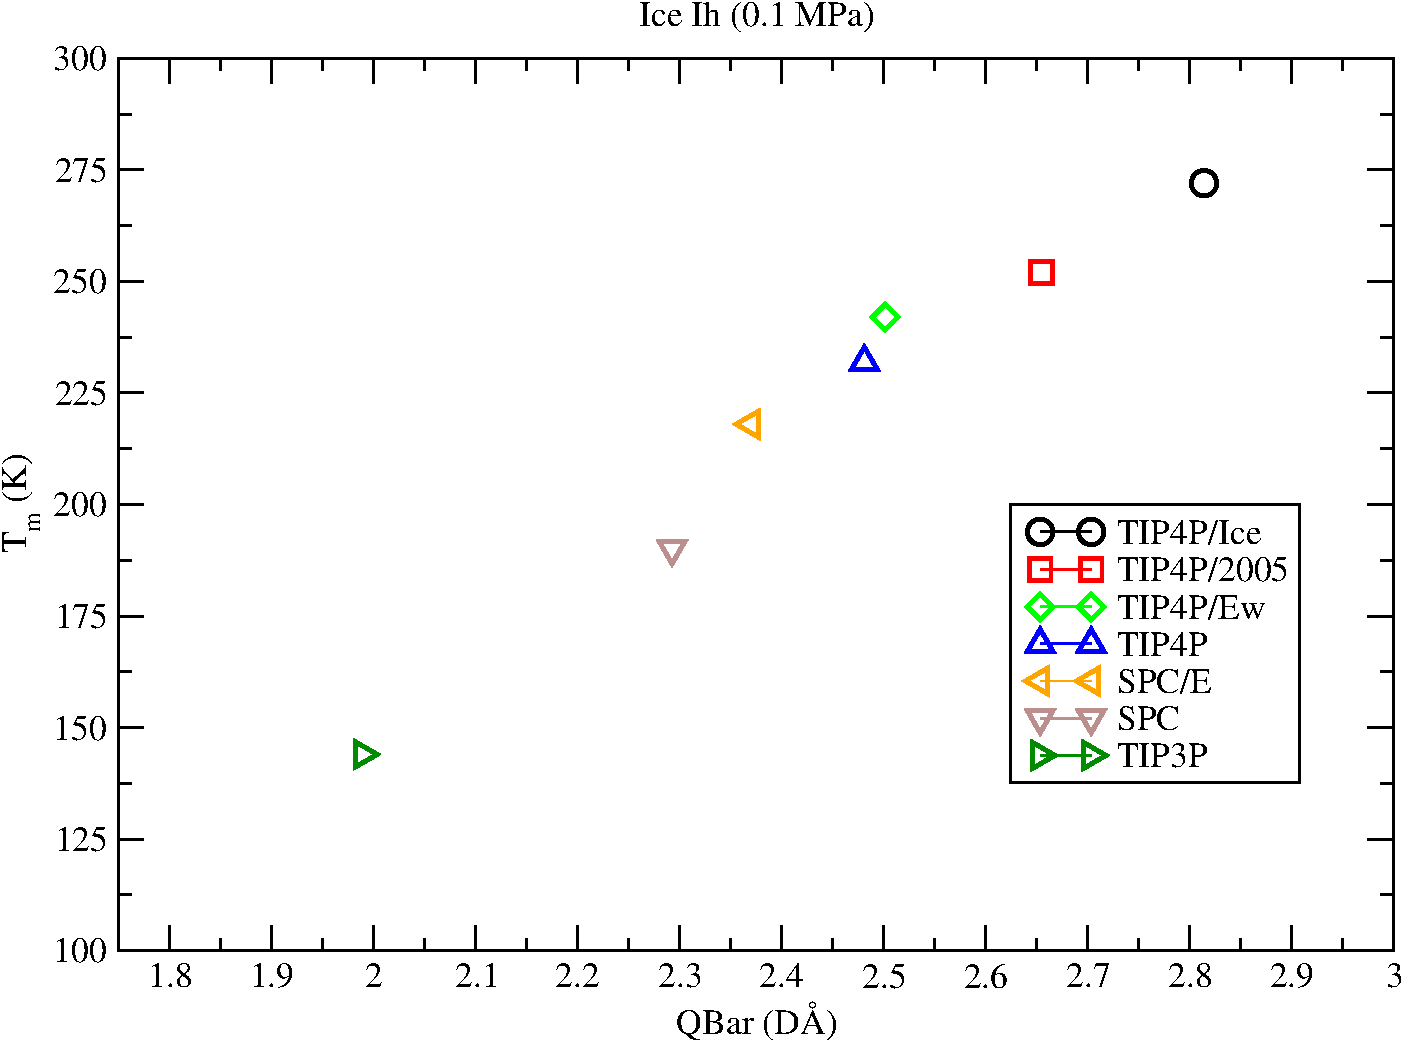
\includegraphics[width=\linewidth]{Figures/Tm_Ih_Qbar_plot.pdf}
\caption{\label{fig:QBar} Melting point for ice-I$_h$ of several
  popular water models as a function of the $\overline{Q}$ for the model. We see
  a strong correlation between a more accurate melting point and a
  larger value of $\overline{Q}$. We estimate that a $\overline{Q}$ of
  approximately 2.8 D\AA$^{2}$~will result in the experimental melting point
  of 273.15 K. A linear regression of the data predicted
  an optimal $\overline{Q}$ to be 2.7690 D\AA$^{2}$~.}
\end{figure*}

\begin{figure*}
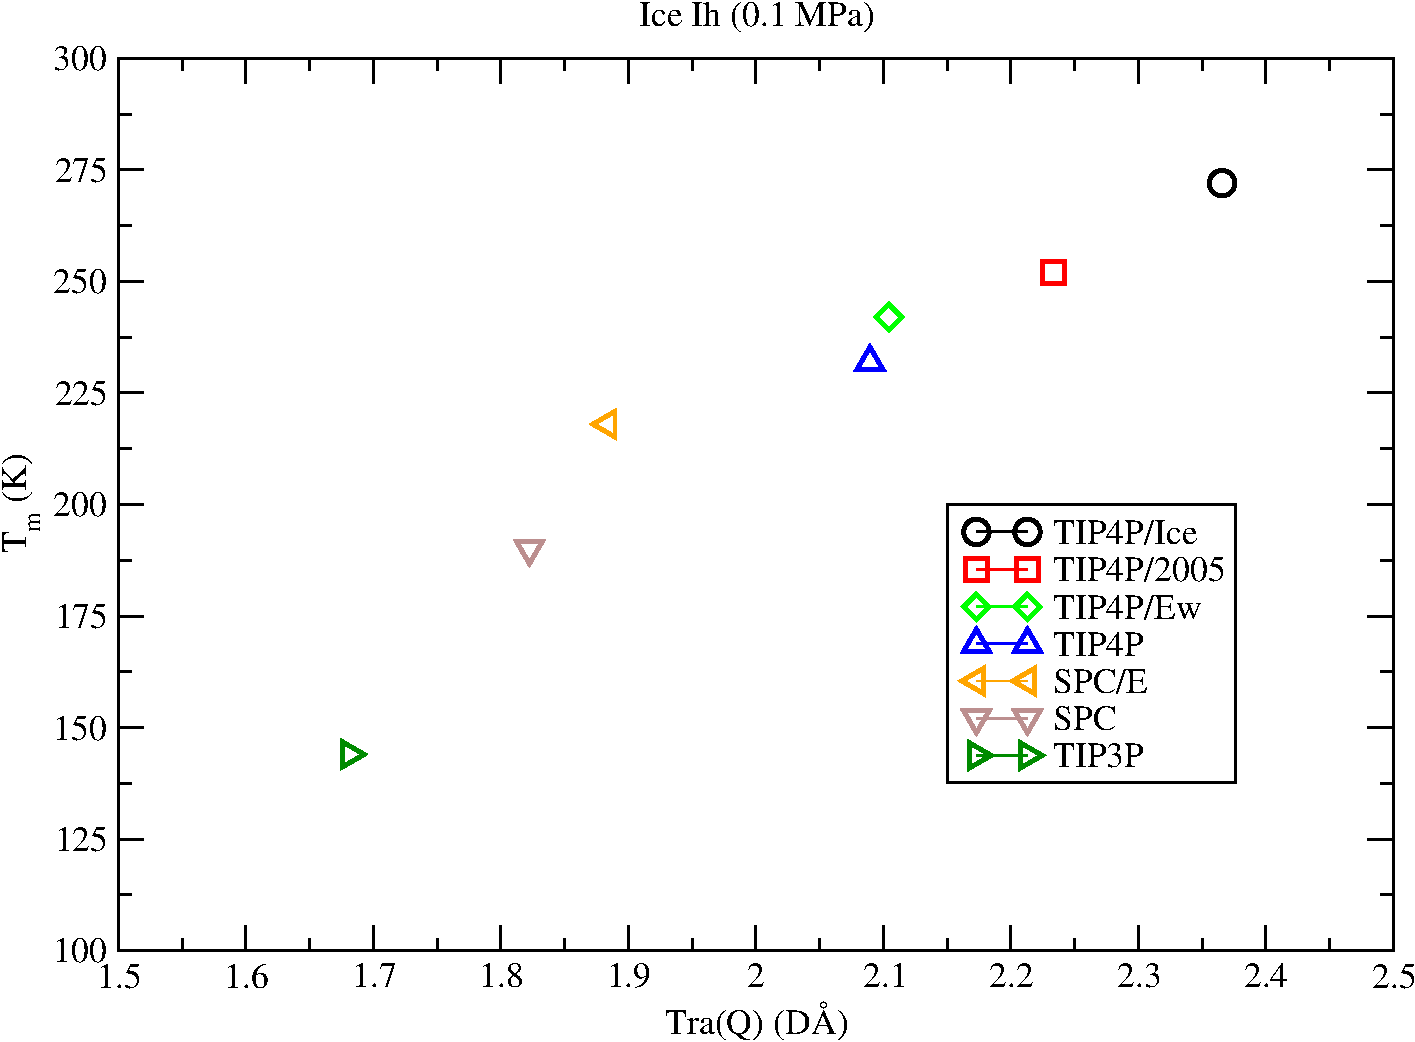
\includegraphics[width = \linewidth]{Figures/Tm_Ih_TraQ_plot.pdf}
\caption{\label{fig:TraQ} Melting point for ice-I$_h$ of several popular water models as a function of the trace of the quadrupole tensor for that model. We see a strong correlation between a more accurate melting point and a larger value of the trace. We estimate that a trace of approximately 2.3 D\AA$^{2}$~will result in an experimental melting point of 273.15 K.}
\end{figure*}

While it is still unclear if these results are indicative of an
experimentally observable phenomenon, exploring correlations such as
this can help in the development of water models in the future. 


\subsection{Transport Properties}
Transport phenomena are processes that describe the transfer (flux) of
mass, heat, momentum, and charge. During this
process, the transferred quantity is conserved, \textit{i.e.}, the
moving quantity is neither created nor destroyed. Because of this, a set
of balance, or conservation equations can be written down describing
the movement of these quantities in the presence of a flux. The set of
balance equations for the transport of mass, energy and momentum are
presented in Table \ref{tab:transport}. 


\begin{table}
	\caption{BALANCE AND CONSTITUTIVE EQUATIONS FOR MASS, ENERGY,
          AND MOMENTUM TRANSPORT\label{tab:transport}}
        \begin{threeparttable}
        \begin{tabular}{rcc}
          \hline \hline
          & \textbf{~~Balance Equations~~} & \textbf{~~Constitutive Equations~~}\\ \hline 
          \textbf{~~Mass~~} & $\frac{\partial c (\vec{r}, t)}{\partial t} + \nabla \vec{j} = 0$ & $\vec{j} = -D \cdot \nabla c(\vec{r}, t)$\\
          \textbf{~~Energy~~} & $C_p \frac{\partial T (\vec{r}, t)}{\partial t} + \nabla \vec{J} = 0$ & $\vec{J} = -\lambda \cdot \nabla T(\vec{r}, t)$\\
          \textbf{~~Momentum~~} & $\rho \frac{D \vec{v}(\vec{r}, t)}{Dt}
                                  + \nabla \overleftrightarrow{\sigma} =
                                  0$ & $\overleftrightarrow{\sigma}_{x,z} = -\eta \cdot
                                       \nabla_z (\rho v_x)$\\ \hline
          \hline
          \end{tabular}
\end{threeparttable}
\end{table}

When a transport flux is present, a characteristic response of the
material will become apparent. For example, in the presence of an
energy flux, a thermal gradient will develop in the
material. Likewise, a momentum flux will cause a velocity distribution
to form in the system. Through a series of constitutive equations
(right column of Table \ref{tab:transport}), it is possible to relate
the flux to the observed system response through a proportionality
constant describing the transport.  Following Fick's Law, the
diffusion coefficient, or diffusivity, ($D$) is the proportionality
constant describing the transport of mass, $\vec{j}$ and the resulting
concentration gradient $\nabla c(\vec{r}, t)$. Similarly, by Fourier's
Law, the thermal conductivity, $\lambda$, is described by the energy
flux $\vec{J}$ and the thermal gradient through the material
$\nabla T(\vec{r}, t)$. Lastly, from Newton's Law of Viscosity, the
shear stress ($\sigma_{x,z}$) and the velocity gradient
$\nabla_z (\rho v_x)$ are related through the shear viscosity
$\eta$. 


% \begin{itemize}
% \item \textbf{Diffusion (Fick's Law):} $\vec{j} = -D \cdot \vec{\nabla}c(\vec{r},t)$ \vspace{0.05in}\\
% The diffusion constant, $D$, relates the mass flux to the concentration gradient.
% \item \textbf{Thermal Conductivity (Fourier's Law):} $\vec{q} = -\lambda \cdot \vec{\nabla} T(\vec{r},t)$ \vspace{0.05in}\\
% The thermal conductivity, $\lambda$, relates the heat flux to the temperature gradient.
% \item \textbf{Viscosity (Newton's Law of Viscosity):} $\sigma_{x,z} = -\eta \cdot \vec{\nabla}_z (\rho v_x)$ \vspace{0.05in}\\
% The shear viscosity, $\eta$, relates the shear stress to the velocity gradient $\left < d(v_x)/dz \right >$.
% \end{itemize}

\subsubsection{Green-Kubo Relations}
In the 1950s, Green and Kubo showed that transport coefficients are
directly related to the time dependence of equilibrium fluctuations of
the system.\cite{Green1954,Kubo1957} If we consider an arbitrary
dynamic property $A(t)$ with a total time derivative of $\dot{A}(t)$,
then the displacement at time $t$ is given by
\begin{equation}
A(t) - A(0) = \int_0^t dt' \dot{A}(t').
\end{equation}
Squaring both sides and averaging over time origins we obtain 
\begin{equation}
\langle [A(t) - A(0)]^2 \rangle = \int_0^t dt'' \int_0^t dt' \langle
\dot{A}(t') \dot{A}(t'') \rangle
\end{equation}
Recognizing that the integrand is symmetric in $t''$ and $t'$, and
that the integral is taken over a square in $t'-t''$ space, we can
integrate over one half the square and double the result. Further, if
we assume the property $\langle \dot{A}(t') \dot{A}(t'') \rangle$ to
be a stationary correlation function, then we are able to shift time
origins without issue. 
\begin{equation}\label{eq:gk}
  \langle [A(t) - A(0)]^2 \rangle = 2 \int_0^t dt'' \int_0^{t''} d\tau ~
  (\tau-0)~\langle \dot{A}(\tau ) \dot{A}(0) \rangle
\end{equation}
Equation \ref{eq:gk} is invariant under interchanging the two
integrations. Lastly, taking a long-time limit collapses one of the
integrals and we are left with a general relation describing the
mean-square displacement of a dynamic quantity and an integral of a
time correlation function.
\begin{equation}\label{eq:gk2}
 \gamma =  \mathrm{lim}_{t \rightarrow \infty} \frac{\langle[ A(t) - A(0)]^2 \rangle}{2t} =
  \int_0^{\infty} d\tau ~ \langle \dot{A}(\tau ) \dot{A}(0) \rangle
\end{equation}
Solving for the transport coefficient ($\gamma$) of interest, is
simply a matter of determining the appropriate dynamic property
$A(t)$, and computing the long-time correlation function. However,
extracting transport coefficients from equilibrium simulations in this
manner is often computationally expensive. The correlation functions
decay slowly, requiring long simulation times.

\subsubsection{Non-equilibrium Molecular Dynamics Methods}
An alternative approach to obtaining transport coefficients is through
the use of non-equilibrium molecular dynamics (NEMD) simulations.
During NEMD simulations, the system is driven out of equilibrium by
the presence of an external perturbation (\textit{e.g.} a thermal or
velocity gradient), and the flux required to sustain the imposed
gradient is computed. Once in-hand, the computed flux and imposed
gradient can be used to obtain the transport coefficient through the
linear constitutive relations in Table \ref{tab:transport}.

For example, if the desired transport property is the thermal conductivity
($\lambda$) of a material, two regions of the simulation box can be
thermostatted, and the kinetic energy flux ($J$) required to maintain
the temperature difference can be calculated. Once this value is
converged, $\lambda$ is be obtained by
\begin{equation}\label{eq:thermalTransport}
J_{z} = - \lambda \big(\frac{\partial T}{\partial z}\big).
\end{equation}
Here, the separation has been taken to be along the $z$-dimension of
the system.  Similarly, the shear viscosity ($\eta$) of a fluid can be
computed by determining the momentum flux ($ j_{z}(p_{x})$) required
to maintain a given average velocity in two spatially separated
regions.
\begin{equation}\label{eq:momentumTransport}
  j_{z}(p_{x}) = -\eta \big(\frac{\partial v_{x}}{\partial z}\big)
\end{equation}

Simulation times to converge the required flux is often shorter than
when computing transport properties using the Green-Kubo
relations. However, computing the appropriate flux can be quite
challenging. Recently, Kuang and Gezelter have developed an approach
to non-equilibrium molecular dynamics based on earlier work by
M\"uller-Plathe, in which they invert the measured and imposed
quantities.\cite{Kuang2010,Kuang2012} In their method, aptly named
reverse non-equilibrium molecular dynamics, the flux is imposed across
two spatially separated regions of the simulation box, and the
gradient response is measured. Again, the desired transport
coefficient can be obtained through a linear constitutive
relation. This method is advantageous over NEMD approaches as the
gradient response of the system is often much easier to measure
than the flux.

%%%%%%%%%%%%%%%%%%%%%%%%
% Water is abundant and found everywhere.
% Water has a lot of weird properties.
% Because of this, ancient humans thought it was important.
% We shall start at understanding the structure of water in each
% phase, then consider coexistence.
%%%%%%%%%%%%%%%%%%%%%%%%
\section{H$_2$O: A Simple Molecule with Complex Behavior}
Water is the simplest compound that can be constructed from the two
most abundant reactive elements in the universe, oxygen and
hydrogen. It is also the second most common molecule in the universe,
trailing behind diatomic hydrogen, $\mathrm{H}_2$.  On Earth, water
occupies nearly $1.4\times 10^{9}~\mathrm{km}^{3}$\cite{Brown2016},
and accounts for 40\% to 70\% of Earth's retention of heat. It is one
of the few molecules that can be found in its solid, liquid, and
gaseous forms at ambient temperatures and pressures.  Some
hypothesize that life cannot exist without water, as all forms of life
found thus far depend on it.\cite{Caldecott2008,Henry2005} In humans,
water composes nearly half the volume of each cell.\cite{Ling2004} It
is the ubiquitous nature of water and ice that gives rise to its
importance; due to its natural abundance a wide variety of chemistry
and physical processes occur within this medium, and at its surface.

In addition to being found everywhere in naturally occurring
abundance, water expresses numerous structural, dynamic, and
thermodynamic anomalies.\cite{Brovchenko2008}. The melting, boiling,
and critical points are unusually high compared to molecules of
similar size. The density of ice increases upon heating (up to
70~K). The density of the liquid increases with increasing temperature
(up to $\sim$ 281 K). Pressure can melt the solid rather than freezing
the liquid, and there are more solid phases than observed for similar
sized molecules. While the principles governing these and other unique
properties of water are not completely known, many of the observed
anomalies are attributed to the electronic distribution around water
and the resulting strength of the hydrogen bond.

% In ancient times, humans recognized the importance of water. Around
% 700 BCE, the Greek philosopher Thales of Miletus, one of the seven
% sages of antiquity, declared that everything was composed of
% water. Later in the 5th century BCE, Empedocles described water as
% being one of four `classical' elements of the ancient world, alongside
% earth, wind, and fire. Likewise, the ancient Chinese described the
% world around them using five elements, earth, wood, metal, fire, and
% water. The importance of water was discovered early in our human
% history, and it has been studied extensively since those early days.

\subsection{The ``Shape'' of Water}
%
% description of what water is? structure constitution etc?
% Gas phase molecule in isolation
% Condensed phase liquid water as collection
% Description of ice and it's structures
%
Defining water's structure can prove a bit challenging. This is mainly
due to the vast number of observed structures and configurations it is
found in. In the liquid, the dynamic hydrogen bond network evolves
rapidly; hydrogen atoms diffuse much more quickly than their
counterpart oxygen atoms due to `bucket-brigade' like motion. In the
solid phase, motion occurs much more slowly. However, motion is
observed around crystalline defects; hydrogens are still exchanged
between oxygens and on slow time scales, reorientation is still
possible. There is also a large diversity in the crystalline
structures of water ice. Over sixteen unique crystal structures
have been observed or predicted\cite{Chaplin2018}, many of which can
be seen in Figure \ref{fig:phaseDiagram}

\begin{figure*}
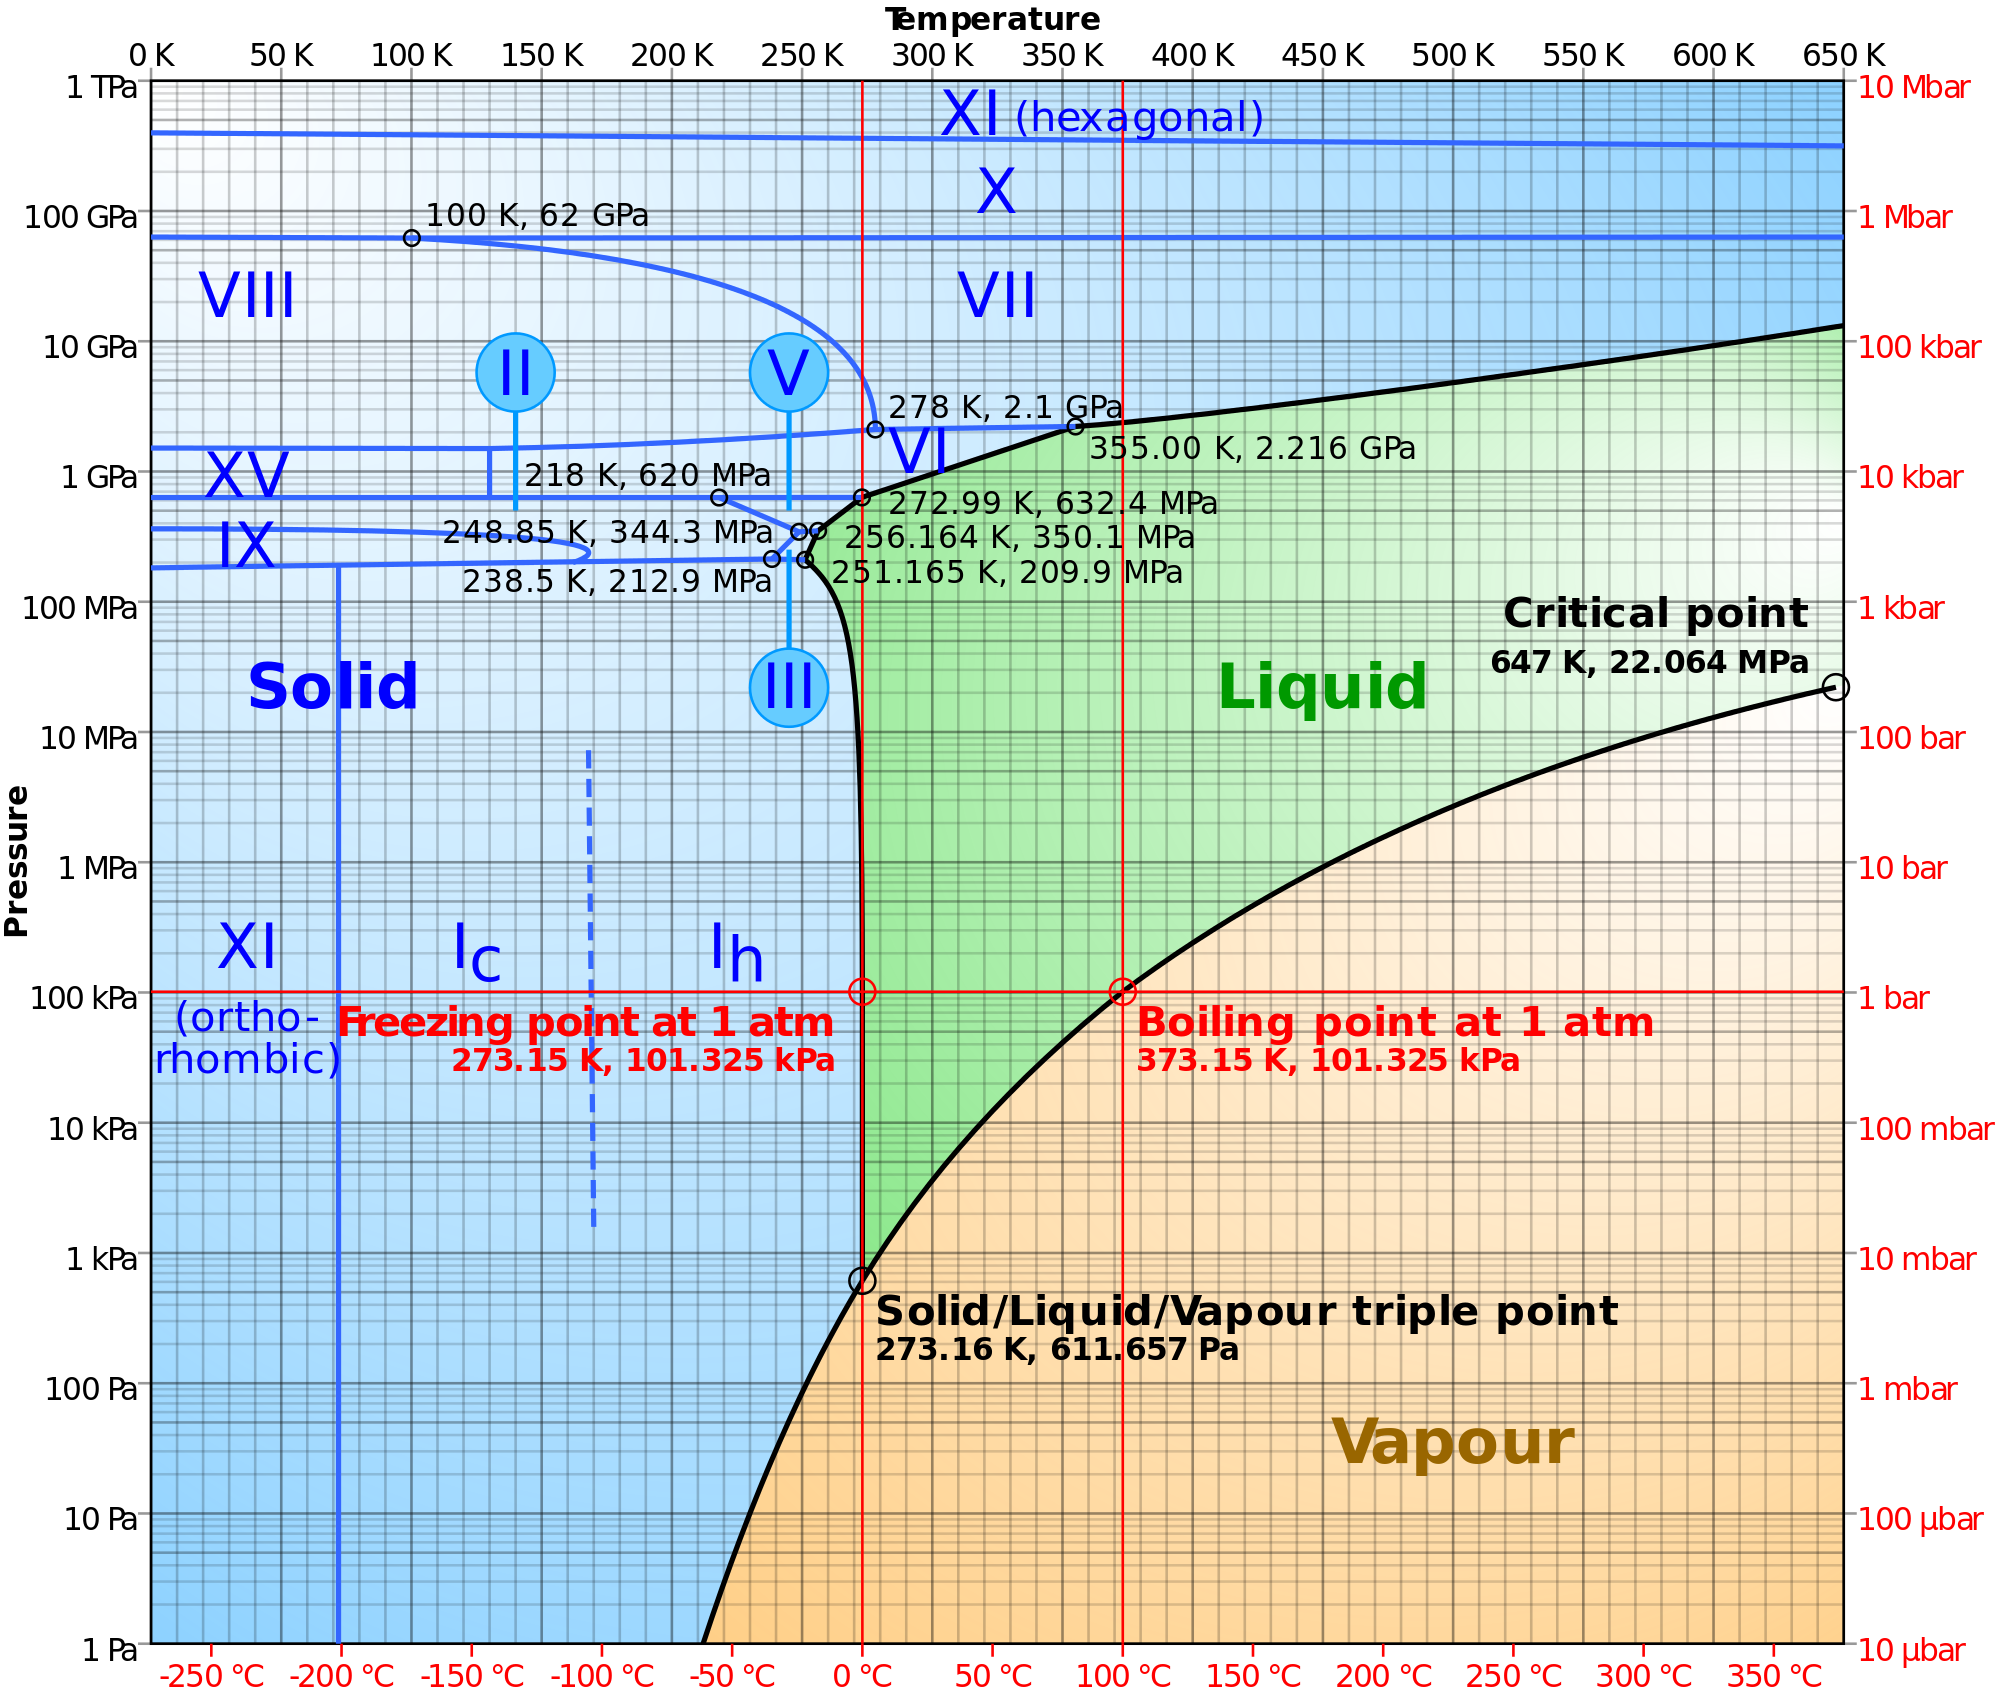
\includegraphics[width=\linewidth]{Figures/PhaseDiagram}
\caption{\label{fig:phaseDiagram} The phase diagram of
  water.\cite{Zhang2015} dT$_{C}$ / dP $<$ 0 at the following boundaries:
  ice-II to ice-V, liquid to ice-I$_\mathrm{h}$, and ice-VII to
  ice-VIII. Conversely, dT$_{C}$ / dP $>$ 0 at the following boundaries:
  liquid to vapor, liquid to ice-(V, VI, VII). dT$_{C}$ / dP $\approx$
  $\inf$ at the ice-(VII, VIII) to ice-X boundary occurring at 60 GPa.
  dT$_{C}$ / dP $\approx$ 0 at ice-I$_\mathrm{h}$ to ice-XI boundary at
  low temperatures. }
\end{figure*}


\subsubsection{Gaseous Water}
In the gas phase, water adopts a `bent' geometry, with an HOH bond
angle of about 104.5\degree~. The oxygen-hydrogen bond length has been
computed with high levels of accuracy to be roughly 1 \AA~ long. These
bond lengths and bend angles are an equilibrium value, as the
molecules are constantly vibrating. Even at $-$273.15~\degree C some
residual motion remains. This is a zero-point energy,
and has considerable implications for the potential energy of the
molecule.

Water's electrons are not symmetrically distributed about the
molecule. This gives rise to higher order multipoles, and it is these
electronic distributions that govern many of water's characteristic
properties. In the gas phase, water has a dipole moment of about
1.85~D. This dipole is highly polarizable, that is, it readily
responds to an external electric field, be it applied or created by
molecules in the local environment. In the condensed liquid phase, the
dipole moment becomes much harder to probe, but values have been
reported ranging from 2.2~D to 2.9~D.


\subsubsection{Liquid Water}
Water is a liquid at room temperature because of its large dipole
moment and the strength of the intermolecular hydrogen bonds. These
bonds are significantly stronger than the van der Waals interactions
arising from the instantaneous polarization of molecules. Numerically,
hydrogen bonds have a strength of about 20
$\mathrm{J}~\mathrm{mol}^{-1}$, about ten times thermal fluctuation at
room temperature. The order of magnitude difference between the
intermolecular interactions and thermal fluctuations means that the
liquid will not boil at room temperatures. The intermolecular forces
for similar size molecules are weaker, for example
$\mathrm{H}_2\mathrm{S}$ boils at -60\degree~C. The strong hydrogen
bonds and the large dipole moment of water holds the molecules
together in a condensed phase at room temperature.

The polarizability of a water molecule leads to another interesting
property, namely, its local bonding environment. In the liquid phase,
water molecules often adopt near-tetrahedral geometries with other
water molecules, resulting in $\sim$~4 nearest neighbors at ambient
conditions. The maximum density of the liquid is observed to occur at
$\sim$~4\degree~C, and cooling further results in decreasing
density. Liquid water transitions to ice when the local ordering
becomes long ranged.


\subsubsection{Water Ice}
%
% Describe crystal structures of ice, examples of where some occur.
% Proton disordered structure, residule entropy. 
%
%Annu. Rev. Phys. Chem. 2017. 68:285–304
Water ice is a fundamental solid, with implications in biological,
environmental, geological, and extraterrestrial
phenomena.\cite{Shultz2017} Biologically, many organisms have adapted
to block advancing ice fronts. These organisms produce antifreeze
proteins which disrupt the hydrogen bonding network at the ice /
liquid interface, preventing further ice growth. The movement of
glaciers has carved out surface features on Earth, and throughout our
solar system reactions and transport of a variety of molecules
occurs at the surface of ice.


% John Finney, A Very Short Introduction to Water. Oxford University
% Press. 
The structure of hexagonal ice (ice-I$_\mathrm{h}$) has been studied
extensively using experimental methods such as neutron scattering and
x-ray spectroscopy, as well as NMR and laser
spectroscopy.\cite{Kuhs2012} In ice-I$_\mathrm{h}$, water molecules form
puckered six member rings, with OOO angles formed by three neighboring
molecules close to 109.5\degree~. These rings can stack on top of one
another and expand to form large sheets, giving rise to the observed
six-fold symmetry of snowflakes. Due to the open structure of the
crystal, it is possible to interweave an equivalent second ice crystal
through the first. These structures have a larger density than the
more open ice, and are aptly named ultra-high density ices. Ice also
crystallizes into cubic structures, although no interwoven lattice has
yet been observed for this geometry. There are currently 16
different crystal structures known for water ice, some of which can be
seen in Figure \ref{fig:phaseDiagram} and Table \ref{tab:iceProps}.

\begin{table}
\centering
\caption{ICE CRYSTAL SYMMETRY AND HYDROGEN ORDERING}
\label{tab:iceProps}
\begin{threeparttable}
\begin{tabular}{lccc}  
\hline\hline 
  ice form & crystal structure & density (g cm$^{-3}$) & proton arrangement  \\ \hline
  I$_\mathrm{h}$ & hexagonal & 0.92 & disordered \\
  I$_\mathrm{c}$ & cubic & 0.93 & disordered \\
  II & rhombohedral & 1.17 & ordered \\
  III & tetragonal & 1.14 & disordered \\
  IV & rhombohedral & 1.27 & disordered \\
  V & monoclinic & 1.23 & disordered \\
  VI & tetragonal & 1.31 & disordered \\
  VII & cubic & 1.50 & disordered \\
  VIII & tetragonal & 1.46 & ordered \\
  IX & tetragonal & 1.16 & ordered \\
  X & cubic & 2.51 & symmetric \\
  XI & orthorhombic & 0.92 & ordered \\
  XII & tetragonal & 1.29 & disordered \\
  XIII & monoclinic & 1.23 & ordered \\
  XIV & orthorhombic & 1.29 & ordered \\
  XV & pseudo-orthorhombic & 1.30 & ordered \\
  XVI & cubic & 0.81 & disordered \\ 
\hline \hline
\end{tabular}
    \begin{tablenotes}
      \small
    \item Data taken from Reference \cite{Chaplin2018}.
\end{tablenotes}

\end{threeparttable}
\end{table}


% Ice Ih at -30 \degree ~C, apply 30,000 atmospheres of pressure
% and we will observe a phase transition to ice-III. Similarly, cool
% ice-III to -40 degrees Celcius and we will see a phase transition to
% ice-II. There are approximately sixteen different known crystal
% structures of ice, each one stable in some unique region of the phase
% diagram. Also, there are ice phases which have been predicted by
% computer simulation which have not yet been observed in vivo. If we
% inspect the phase transition from ice-Ih to ice-III closer, we will
% see a distortion in the crystalline geometry under the large pressure
% conditions. Some of the puckered six-membered rings will compress into
% five-membered structures, resulting in a more dense packing of water
% molecules. However, this will place more strain on the
% hydrogen-bonds. In ice-III, the OOO bond angles vary between 88
% degrees and 148 degrees. Likewise, the hydrogen-bond lengths will also
% change under this distortion. In ice-Ih, hydrogen-bonds are typically
% 0.276 nm, in ice-III hydrogen-bonds are found between 0.271 nm and
% 0.283 nm.

In 1933, Bernal and Fowler established a set of rules for populating
hydrogens into an oxygen ice lattice.\cite{Bernal1933} These rules are
as follows; each oxygen atom is covalently bonded to two hydrogens,
and each hydrogen in each water molecule forms a hydrogen bond with
one other oxygen. This means there is exactly one hydrogen between
every two oxygen sites in the lattice. The result of these rules is
that each oxygen is in a tetrahedral environment, and is donating two
hydrogens and accepting two hydrogen bonds.

Following these ice-rules, we see that there are two \textit{kinds} of
crystals that can be formed, \textit{ordered} and
\textit{disordered}. In the \textit{ordered} case, the hydrogen
configurations for equivalent water molecules in all unit cells are
the same, whereas in a \textit{disordered} ice the proton
configurations are unequivalent. We can describe these lattices as
being orientationally ordered or disordered, however, they are more
commonly described in terms of their proton ordering. The two
descriptions are equivalent as the arrangement or ordering of the
hydrogens gives rise to the orientation of the water molecules.  Ices-
I$_\mathrm{h}$, III, IV, V, VI, VII, XII, XVI are proton disordered,
while Ices- II, VIII, IX, and XI are proton ordered.

Upon cooling, ice-III and ice-VII undergo a phase transition to
ordered forms, ice-IX and ice-VIII respectively. Transitions of proton
disordered ice to proton ordered ice must inherently involve the
reorientation of water molecules, the transfer of
hydrogens, or some combination of the two. However, if all molecules
in the lattice satisfy the Bernal Fowler ice-rules, any one water
molecule reorientation or proton transfer will inevitably break the
ice-rules. Therefore, we conclude these events must happen in concert,
large collections of molecules must simultaneously undergo some
combination or reorientation and proton transfer. However, the energy
required to do so would be quite large, and larger still for
increasing number of molecules involved. This amount of energy is not
likely available at the thermal conditions where these transitions are
observed to occur, therefore, it is believed that the these
transitions must depend on defects within the lattice.

There are two known kinds of defects in ice
lattices, \textit{orientational} defects, known as Bjerrum defects,
and \textit{ionic} defects. There are two kinds of Bjerrum defects,
D-defect (from the German \textit{doppelbesetze} meaning doubly
occupied), and an L-defect (from \textit{leere} meaning empty). A
D-defect occurs when there are two hydrogens between two neighboring
oxygens, and an L-defect occurs when there are no hydrogens between
the oxygen sites. These are of course in violation of the Bernal
Fowler ice-rules, however, they act as proton sinks and sources when
the crystal undergoes phase transitions from proton disordered to
proton ordered. Ionic defects form when a proton transfer happens
between two oxygens, resulting in the formation of a hydroxide and
hydronium ion.

% Residual Entropy of ice.
\vspace{0.6cm}
\begin{flushleft}
\textit{Residual Entropy of Ice}
\end{flushleft}

If we further consider the Bernal Fowler ice-rules, we see that the
hydrogen arrangement in ice-I$_\mathrm{h}$ is not unique. In 1935,
Linus Pauling argued that any arrangements of hydrogens which
satisfies the ice-rules is valid and has equal probability of
occurring since each unique arrangement has the same energy,
\textit{i.e.} they are degenerate configurations. Due to this, he
predicted ice-I$_\mathrm{h}$ to have a \textit{residual entropy}, that is, a
non-vanishing positive entropy ($S_{0}$) at zero Kelvin. This entropy
can be computed from Boltmann's equation of statistical mechanics,
\begin{equation}\label{eq:Boltzmann-W}
S = k_{B}~\mathrm{ln}(W)
\end{equation}
where $k_{B}$ is Boltzmann's constant and $W$ is the number of
equivalent arrangements of the molecules. Pauling estimated the number
of configurations in two separate ways.\cite{Pauling1935} First, we
must recognize that there are six possible ways to orient a water
molecule within a tetrahedral structure formed by neighboring
molecules while satisfying the ice-rules. If we give each water
molecule one of these six orientations at random, there is then a 1/2
probability of having a hydrogen between two oxygens, thus there is a
1/4 chance that there is exactly one hydrogen between every two
oxygens in the lattice. The resulting number of correct possible
arrangements of $N$ water molecules is
\begin{equation} \label{eq:Pauling-1}
W_{Pauling} = (6/4)^{N} = (3/2)^{N}.
\end{equation}   
Pauling arrived at the same result by a second construction. If we
 only enforce there to be a single hydrogen
between each oxygen in the lattice, there are $2^{2N}$ configurations
(since there are $2N$ bonds in the network). For each oxygen atom,
there are $2^{4} = 16$ possible arrangements for the hydrogens, 10 of
which are ruled out as they result in non-intact
molecules. That is, they form structures of (H$_{4}$O)$^{2+}$,
(H$_{3}$O)$^{+}$, (HO)$^{-}$, and O$^{2-}$. Therefore, there are only
6/16 possible configurations allowed for placing hydrogens around each
oxygen. This gives a total number of configurations as,
\begin{equation}
W_{Pauling} = 2^{2N}(6/16)^{N} = (3/2)^{N}.
\end{equation}
Using these results with Equation \eqref{eq:Boltzmann-W}, the residual
entropy follows as
\begin{equation}
S_{0} = k_{B}N\mathrm{ln}(3/2) = R\mathrm{ln}(3/2)
\end{equation}
where $R$ is the molar gas constant,
$R = 8.31447~\mathrm{J~mol}^{-1}~\mathrm{K}^{-1}$. This gives a
residual entropy of
\begin{equation}
  S_{0} = 3.3712~\mathrm{J~mol}^{-1}~\mathrm{K}^{-1} = 0.80574~\mathrm{cal~deg}^{-1}~ \mathrm{mol}^{-1}.
\end{equation}
The residual entropy has been further investigated by Berg \textit{et
  al.} who obtained
$S_{0} \approx 0.81550 \pm 0.00021~\mathrm{cal~deg}^{-1}
~\mathrm{mol}^{-1}$ by means of multicanonical
simulations.\cite{Berg2007} This result was found to be in good
agreement with a series expansion method by Nagle \textit{et
  al.}\cite{Nagle1966}, as well as Giaque and Stouts calorimetry
experiments which estimated
$S_{0} = 0.82 \pm 0.05~\mathrm{cal~deg}^{-1}
~\mathrm{mol}^{-1}$.\cite{Giaque1936}
% end Residual Entropy of ice.


\subsection{Ice / Water Coexistence}
%%%
% General introduction to ice/water coexistence
% Early work in the field, quiescent systems and measures of
% interfacial width.
% Problems discovered specific to ice/water coexistence, improper
% treatment of the electrostatics, coexistence temperatures, etc.
%
%%%

Understanding the ice / water interface is essential for explaining
complex processes such as nucleation and crystal
growth,\cite{Han1992,Granasy1995,Vanfleet1995} crystal
melting,\cite{Weber1983,Han1992,Sakai1996,Sakai1996a} and some
fascinating biological processes, such as the behavior of the
antifreeze proteins found in winter
flounder,\cite{Chapsky1997,Wierzbicki2007} and certain terrestrial
arthropods.\cite{Duman2001} Haymet \textit{et al.}  have done extensive
work on ice-I$_\mathrm{h}$, including characterizing and determining
the width of the ice/water interface for the SPC,\cite{Karim1990}
SPC/E,\cite{Gay2002,Bryk2002} CF1,\cite{Hayward2001,Hayward2002} and
TIP4P~\cite{Karim1988} models for water.  More recently, Haymet
\emph{et al.} have investigated the effects cations and anions have on
crystal nucleation.\cite{Bryk2004,Smith2005,Wilson2008,Wilson2010}
Nada \textit{et al.}  have also studied ice/water
interfaces,\cite{Nada1995,Nada2000,Nada2003a,Nada2012} and have found
that the differential growth rates of the facets of ice-I$_\mathrm{h}$
are due to the the reordering of the hydrogen bonding network at the
interface.\cite{Nada2005}


% Benet, MacDowell, Sanz, PCCP 2014, 16, 22159
% A study of the ice/water interface using the TIP4P/2005 water model

The interfacial free energy between ice and water, $\gamma_{iw}$, is a
crucial parameter for ice nucleation and crystal
growth.\cite{Pruppacher1967,Pruppacher1995} Experimentally obtained
values of $\gamma_{iw}$ range from 25 to 35
$\mathrm{mN}~\mathrm{m}^{-1}$.\cite{Pruppacher1995} This spread stems
from the problem that there are no current methods for obtaining a
robust measurement. Computer simulations have attempted to quantify
$\gamma_{iw}$, and predictions have been made for a series of water
models, some with\cite{Davidchack2012} and some
without\cite{Handel2008} taking full electrostatic interactions into
account. These studies used a variant of the cleaving
method,\cite{Broughton1986} and estimated $\gamma_{iw}$ using the
TIP4P, TIP4P-Ew, and TIP5P-E water models.

Previously, $\gamma_{iw}$ has been estimated using the TIP4P/2005
water model and the method proposed by Bai and Li, studying the
crystal-melt interface of a Lennard-Jones system.\cite{Bai2006} In the
method of Bai and Li, the critical size of crystalline clusters are
measured, and by extension of classical nucleation theory
$\gamma_{iw}$ can be obtained.\cite{Volmer1926,Becker1935} This result
produces an orientationally averaged estimate of $\gamma_{iw}$, which
does not provide any information on the dependency of $\gamma_{iw}$ on
the orientation of the crystal.

Benet \textit{et al.} have measured the interfacial free energy of
ice-I$_\mathrm{h}$ in coexistence with liquid water at 248.5~K by
using the TIP4P/2005 water model by analyzing the spectrum of
capillary fluctuations at the interface.\cite{Benet2014} This method
was originally described by Hoyt \textit{et al.}\cite{Hoyt2001}, has
been used to calculate the interfacial free energy of hard
spheres,\cite{Davidchack2006} the Lennard-Jones
potential,\cite{Morris2003} and dipolar fluids.\cite{Wang2013}

% In this method, water molecules were labeled as ice-like or
% liquid-like based on local bond order parameters. Next, a discretized
% profile parallel to the interface (i.e, along the $x$ dimension),
% $h(x_{n})$, was computed for many small bins across the system. These
% resulting profiles were then Fourier-transformed,
% \begin{equation}
% h_{q} = \frac{1}{N}\sum_{n=1}^{N} h(x_{n})e^{iqx_n}
% \end{equation}
% giving an amplitude $h_{q}$ for each wave vector $q$, for each of the
% $N$ total bins across the $x$-dimension. 

% Capillary wave theory provides a relationship between these wave
% vector amplitudes and the interfacial stiffness, $\sigma$ by
% \begin{equation}
% \langle |h_{q}|^{2} \rangle = \frac{k_{B}T}{A \sigma q^{2}}
% \end{equation}
% where $A$ is taken to be the product of the two simulation box
% dimensions not normal to the interface. Since the interfacial
% stiffness is dependent on both the crystal plane that is exposed to
% the liquid and the direction which the wave vector propagates, we have
% \begin{equation}
% \sigma = \bigg(\gamma (\theta ) + \frac{d^{2}\gamma (\theta )}{d\theta
% ^{2}} \bigg)_{\theta = 0} .
% \end{equation}
% Here, $\theta$ is the angle between the average planar ice / water
% interface, and the normal vector of the instantaneous interface. The
% orientational dependence of the interfacial free energy can be written
% as an expansion of the Spherical Harmonics\cite{23}, and will be
% unique for each crystal plane studied. 

Benet found an orientationally averaged interfacial free energy of
$27 \mathrm{mN}~\mathrm{m}^{-1}$, which agrees well with recent
estimates using size cluster analysis by Sanz \textit{et
  al.}\cite{Sanz2013}. Benet \textit{et al.} were able to estimate the
free energy of different planes (in coexistence with liquid), and
obtained values of 27 $\pm$ 2, 28 $\pm$ 2, and 28 $\pm$ 2
$\mathrm{mN}~\mathrm{m}^{-1}$ for the $\{0001\}$ (basal),
$\{10\bar{1}0\}$ (prismatic) face, and $\{11\bar{2}0\}$ (secondary
prismatic) faces, respectively. They also observed an interfacial
thickness of about four to five molecular diameters, which was found
to be insensitive to the crystal face exposed to the liquid. Lastly,
when the basal face is exposed to the liquid, they observed local
areas of hexagonal ice and cubic ice within the interface. This
observation is not unique to this study, other simulations and
experiments have shown hexagonal ice to grow with a mixed
I$_\mathrm{c}$-I$_\mathrm{h}$
stacking.\cite{Malkin2012,Moore2011,Seo2012,Carignano2007,Rozmanov2011}
%end Benet, MacDowell, Sanz, PCCP 2014, 16, 22159



\subsection{The Surface Premelting of Ice and the Quasi-Liquid Layer}
% 2. Driving force for the QLL, not unique to ice. Interesting on ice
% because ice occurs everywhere in the universe, therefore, lots of
% interesting things happen at ice surfaces.
% 3. Experimental and theoretical measures of the QLL, who and how have
% studied it.
% 3a. QLL width
% 3b. QLL structure, dynamics
% 4. Observed oddity of friction on ice surfaces is small, transition to
% next subsection where we will talk about friction studies on ice surfaces.

In order to characterize the surface premelting of ice, we must first
understand the crystal termination. While a large
variety of computational and experimental techniques have been used to
probe the structure, dynamics, and properties of this liquid-like
surface film, much is still unknown. Open questions include: at zero,
or small temperatures, are the protons at the surface ordered or
disordered, and does this change with appreciable temperature? Also,
what contribution does this liquid-like layer play in the observed
small friction coefficients commonly found for ice?

\subsubsection{Hydrogen Order at the Surface of Ice}
It is well understood that the formation of a surface requires
considerable energy, and that the molecules at the surface have
interesting characteristics unique to their local
environment. Termination of the repeating crystal lattice results in
undercoordinated molecules which have enhanced mobility at appreciable
temperatures due to the reduced potential experienced at these
sites.

For most materials, crystal surfaces are often defined by the surface
plane relative to the internal coordinates. Ice-I$_\mathrm{h}$
crystals commonly expose the $\{0001\}$ (basal) and $\{10\bar{1}0\}$
(prismatic) faces, although, this does not completely define the
surface as compared with simple solids. Due to the residual entropy of
the proton distribution within the ice lattice, termination of the
crystal along the desired plane but at varying locations throughout
the crystal can result in differential hydrogen patterning at the
surface. The possible proton arrangements could alter the surface
energy ($\gamma$), a thermodynamic quantity that affects crystal growth and
controls crystal shape.

Fletcher was the first to consider proton ordering at
ice-I$_\mathrm{h}$ surfaces, using classical electrostatics arguments
to suggest that the lowest energy surface should be proton
ordered.\cite{Fletcher1992} His arguments stemmed from dipole
interactions among nearest neighbor OH bonds, which also led to the
prediction that the basal surface would undergo a proton ordered to
disordered transition at $\sim$~30~K, and similarly the prismatic
would transition at $\sim$~70~K.

More recently, Buch \textit{et al.} compared basal surfaces with
varying proton arrangements using the TIP4P/Ice and EMP water
models.\cite{Buch2008} They also found that proton ordered surfaces
were of lower energy as compared to disordered states, and observed
alternating rows of proton-exposed and oxygen-exposed termination to
be the most stable.  Pan \textit{et al.} performed density-functional
theory (DFT) calculations on the basal and prismatic surface of an
ice-I$_\mathrm{h}$ and obtained similar surface energies for the two
faces.\cite{Pan2010} However, they observed a strong dependence for
the surface energy on the proton ordering, which was found to account
for up to 50~\% of the total surface energy (significantly larger than
proton ordering in the bulk $<$ 1~\%). This suggests that the ice
surface's thermodynamic ground state will be proton ordered, even for
temperatures well above the bulk order-disorder temperature of about
72~K.

The surface energies for an antiferroelectric ice, ice-XI, were found
to converge with varying exchange-correlation functionals on a value
of about $\gamma_{basal}^{XI} \sim 11~\mathrm{meV~\AA^{-2}}$. However,
the surface energies for ice-I$_\mathrm{h}$ were observed to be spread
over a much larger range of values, from 12.2 to 18.2~
$\mathrm{meV~\AA^{-2}}$. This indicates that for a constant internal
ice-I$_\mathrm{h}$ lattice, slight changes in proton ordering at the
surface can result in large differences in surface energy.

Pan \textit{et al.} investigated surface oxygen
positions. \cite{Pan2010} Due to the crystal termination, these oxygen
atoms could deviate from their lattice positions with thermal
energy. For ice-I$_\mathrm{h}$ surface bilayers, they find the
oxygen-oxygen distance does not change much compared to the bulk. The
average surface oxygen-oxygen distance is 0.02 \AA~ greater than found
in the bulk. This is consistent with experimental results, indicating
distances of 2.77 \AA~ for surface and 2.76 \AA~ for bulk at
38~K.\cite{Parent2002}

Due to the ring stacking structure of ice-I$_\mathrm{h}$, the basal
face could terminate as either a monolayer or a bilayer. Materer
\textit{et al.} studied an ultrathin ice surface exposing the basal
face grown on a Pt(111) substrate at 90K (well below surface melt)
using low-energy electron diffraction (LEED) spectroscopy, in
conjunction with total-energy calculations and molecular dynamics
simulations.\cite{Materer1995,Materer1997} Their results suggested the
basal face is terminated with a full bilayer of molecules, and not a
half bilayer as some had previously conjectured. The same surface
structure was observed later by Braun \textit{et al.}\cite{Braun1998}
and Glebov \textit{et al.}\cite{Glebov2000} using helium atom
scattering experiments at 30K.

\subsubsection{Driving Force of the Surface Premelting}
All crystalline materials exhibit a surface premelting at temperatures
approaching their melting point. Valkealahti and Nieminen observed
surface premelting for an argon crystal below its bulk melting
point.\cite{Valkealahti1987} They found a trend between the the
coordination number of the surface atoms with the onset temperature of
the premelt. Similarly, Starikov and Stegailov observed surface
premelting for iron and aluminum, and investigated the pressure and
temperature dependence of the surface premelt.\cite{Starikov2009}

It is generally accepted that the surface premelt is driven by the
reduced potential experienced by molecules at the surface. This
reduction in potential stems from the undercoordination of the surface
molecules.  At temperatures considerably below the melting point,
these molecules reside in their lattice positions. However, as thermal
energy increases the internal vibrational and rotational modes of the
surface molecules becomes populated. At some critical temperature
(T$^\mathrm{*}$ $<$ T$_\mathrm{m}$), the surface molecules have
sufficient energy to leave their lattice positions and translate along
the surface. This motion is driven by the molecule's ability
to better maximize their intermolecular interactions with their
neighbors. These surface molecules are collectively referred to as a
quasi-liquid layer (QLL), as their structure and properties reflect
some of their condensed liquid phase counterparts, but are distinctly
unique.

\subsubsection{Investigations of the Quasi-Liquid Layer}
% Ice Surfaces by Mary Jane Shultz, Ann Rev Phys Chem
Significant evidence has been given indicating the existence of a
surface premelt quasi-liquid layer on ice. Investigations have been
performed using glancing angle X-ray\cite{Lied1994, Dosch1995},
SFG\cite{Wei2001}, He atom scattering\cite{Suter2006}, atomic force
microscopy\cite{Goertz2009,Doppenschmidt2000},
ellipsometry\cite{Furukawa1997}, photoelectron
spectroscopy\cite{Bluhm2002}, nuclear magnetic resonance
(NMR)\cite{Dec2009,Dec2012}, computational
techniques\cite{Conde2008,Neshyba2009,Gladich2011,Pfalzgraff2011,Gladich2015,Park2010,Shepherd2012,Limmer2014,Persson2015}
and differential interference
contrast\cite{Sazaki2012,Asakawa2016,Sazaki2013} all point towards a
surface premelt. However, there is a large spread in reported onset
temperatures, from 200~K to 260~K. Since each technique probes
different properties of the surface molecules, the observed onset
temperature of the QLL is dependent on the temperature at which those
properties deviate from their solid values. Surface techniques which
probe structural changes tend to be more sensitive and usually suggest
lower temperatures for the onset of the premelting. In contrast to
this, techniques which probe bulk properties of the film require a
larger number of molecules for signal generation, and tend to yield
warmer temperatures for the onset. Also, many have argued that small
amounts of contamination could result in drastically varying
results.\cite{Elbaum1993,Wettlaufer1999} Given all of this, the
commonly compared against onset temperature for the QLL is around
243~K.

While there is general agreement on the existence of a
surface premelt, there is considerable disagreement about its
characteristics. Henson \textit{et al.} predicted that the QLL should
behave as a supercooled water\cite{Henson2005}, while Goertz
\textit{et al.}  measured the adhesive and mechanical properties of
the QLL, showing it to be viscoelastic in nature.\cite{Goertz2009}
More recently, Suzuki \textit{et al.}  have probed the QLL with
differential interference contrast and observed two separate immiscible
liquid water films.\cite{Sazaki2012,Asakawa2016,Sazaki2013} Again
these differences may arise due to the particular probe used to
measure the quasi-liquid layer. However, amongst the disagreements
there resides fruitful observations which may help us to elucidate
the nature of this interesting phenomenon. 

\vspace{0.6cm}
\begin{flushleft}
\textit{Formation of the Quasi-Liquid Layer}
\end{flushleft}

Sum frequency generation (SFG) spectroscopy is able to probe the
orientational disorder of molecules at a surface. The basal surface of
ice-I$_\mathrm{h}$ is known to present dangling or `free' O-H bonds
normal to the interface. The orientational order of these dangling
bonds can be probed using SFG spectroscopy, and observing the
temperature at which the intensity of the SFG signal decreases can
estimate the onset of the QLL.

Wei \textit{et al.} have probed the O-H bonds at the basal surface
using SFG spectroscopy for temperatures between 173~K and
271~K.\cite{Wei2001,Wei2002} They observed that the disorder became
apparent as the temperature approached 200~K, and increased with
warmer temperatures.  These results indicate that the structural
ordering decreases in a continuous fashion from bulk ice to the
liquid-like layer, which also agrees well with results from proton
channeling and glancing-angle X-ray
scattering.\cite{Golecki1978,Dosch1995} Using molecular dynamics
simulations, Ikeda-Fukazawa and Kawamura also observed water molecules
with large vibrational and rotational motions on a basal surface of an
ice-I$_\mathrm{h}$ crystal at the same
temperatures.\cite{Ikeda-Fukazawa2004} Their results supported the
continuous transition of structural ordering across the qausi-liquid
layer.

In contrast, simulations by Kroes \textit{et al.}  predicted the
melting occurs in a bilayer-to-bilayer manner.\cite{Kroes1992} Using
the TIP4P potential, he observed a sudden transition in the
polarisation of the surface between 210~K and 230~K.  The step-wise
surface melting was recently observed by Sanchez \textit{et al.};
using SFG spectroscopy, they probed the hydrogen-bonded OH stretch
frequency between temperatures of 235~K and 273~K.\cite{Sanchez2017}
They observed a sudden increase in the width of the surface premelt
around 257~K, which occurs in a bilayer-by-bilayer manner. 

\vspace{0.6cm}
\begin{flushleft}
\textit{Width of the Quasi-Liquid Layer}
\end{flushleft}

Using molecular dynamics simulations, Benet \textit{et al.} studied
the fluctuations at the ice / quasi-liquid layer, and the quasi-liquid
layer / vapor interfaces.\cite{Benet2016} Using a structural order
parameter, they estimated the width of the surface premelt to be
$\sim$ 0.9~nm, agreeing with other computational
predictions\cite{Conde2008,Bishop2009,Pan2011} and experimental
observations of Bluhm \textit{et al.}\cite{Bluhm2002}, Beaglehole and
Wilson\cite{Beaglehole1993}, and Murata \textit{et
  al.}\cite{Murata2015}. Close to the triple point (2~K below it),
Benet found that the surface premelt of the prismatic face behaves as
two independent interfaces. They also observed that the two interfaces
fluctuated independently of one another, and the QLL / vapor interface
behaved almost indistinguishably like a bulk-water / vapor interface.

Conde \textit{et al.} performed an in-depth analysis of the surface
premelt using the SPC/E, TIP4P, TIP4P/Ice, and the TIP4P/2005 water
models for the basal, prismatic, and secondary prismatic surfaces of
an ice-I$_\mathrm{h}$ crystal.\cite{Conde2008} They found that when
compared at the same temperature of undercooling relative to the
model's melting point, each model predicted the same width of the
quasi-liquid layer. In addition, they observed facet dependent onset
temperatures for the quasi-liquid layers. This agreed well with 
optical reflection experiments, which showed a temperature
dependence of the QLL thickness with the exposed
crystal facet.\cite{Elbaum1993} 

Understanding the onset temperatures of the quasi-liquid layer for the
different facets of ice-I$_\mathrm{h}$ is necessary for understanding
crystal growth.  Ice crystals grown from bulk vapor change
morphologies as the temperature is cooled below the triple
point. Plates and columns are observed to alternate as the dominant
structure, and dendrites have been observed at high
saturations.\cite{Libbrecht2005} These varying crystal structures are
attributed to a crossover in the growth rates of the basal and
prismatic faces. However, we do not currently understand what
structural transformation occurs at the surface to drive the
crossover.\cite{Libbrecht2005,Furukawa2007,Liu1996} Kuroda and Lacmann
have attributed the crossover to differential QLL formation
temperatures for different exposed crystal facets.\cite{Kuroda1982}



\subsubsection{Anisotropic Diffusion of the QLL}
While probing the dynamics of molecules in the quasi-liquid layer,
Pfalzgraff, Neshyba, and Roeselova observed anisotropic diffusion on
the surfaces of the prismatic, 14\degree~ and 28\degree~ pyramidal
facets.\cite{Pfalzgraff2011} They attributed this anisotropy to the
underlying surface features. The prismatic and pyramidal surfaces
present large channels to the QLL, and the energy required for
diffusion along the channel was conjectured to be smaller than
traversing across. The basal face also presents a non-uniform surface
to the QLL, although isotropic diffusion was observed. They argued
that the barrier for diffusion in each of the non-uniform directions
on this surface was much closer in energy, and readily available for
molecules at the simulated temperature.

In a follow up study, Gladich \textit{et al.} investigated the
temperature dependence of this anisotropic diffusion, and found at low
temperatures that movement normal to the interface happened in concert
with large displacements in the normal plane, even when the normal
motion was still well within the QLL.\cite{Gladich2011} They concluded
that these motions normal to the interface will largely influence
surface diffusion of the molecules. These motions were in good
agreement with the diffusion mechanism proposed by Bishop \textit{et
  al.}\cite{Bishop2009} and by Bolton and Pettersson\cite{Bolton2000},
which suggested the outermost molecules of the QLL moved across a
relatively rigid surface. Diffusion characterized in this way is
highly sensitive to the underlying surface morphology and topography.
That is, if the surface geometry or potential energy surface for
diffusion is anisotropic, we should expect to recover non-uniform
diffusion across the surface.

Observations that in-plane diffusion follows motions transverse to the
interface were observed at warmer temperatures as well. However, at
warm enough temperatures isotropic diffusion was
observed.\cite{Gladich2011,Gladich2015} Gladich \textit{et al.}
proposed the following mechanism and reported activation
energies. Through vertical motion, the QLL molecule leaves a
well-hydrated local environment close to the ice surface, moving to
the outer portion of the surface where there are fewer hydrogen bond
partners. Gladich concluded that the activation energy for
high-temperature diffusion is greater than that of the
low-temperature. This is due to the thicker surface premelt at warmer
temperatures.  They further estimated these activation energies to be
29.1 kJ mol$^{-1}$ for low-temperature diffusion (approximately the
energy of one hydrogen bond with the NE6 model), and 53.8 kJ
mol$^{-1}$ at temperatures close to the melting point (roughly two
hydrogen bonds).  However, with increasing temperature and a thicker
surface premelt, the surface morphology and topography is masked and
isotropic diffusion is recovered. Gladich observed the recovery to
isotropic diffusion between 49~K and 39~K of undercooling for the NE6
model.

The diffusion coefficients computed by Gladich \textit{et al.} also
agreed well with the surface diffusivity measurements by Nasello
\textit{et al.}, who observed the formation of grain boundaries on
polycrystalline ice surfaces.\cite{Nasello2007} Interestingly, the
diffusion coefficients also agreed with NMR measurements of
supercooled water by Price \textit{et al.}, especially at warmer
temperatures. \cite{Price1999} At cooler temperatures ($\sim$~240~K),
the reported values deviate from one another. Simulations of bulk
liquid also agree with the work of Price, however, at colder
temperatures the bulk-liquid simulations predict a negative Arrhenius
curvature, opposite of that observed by
Price.\cite{Picaud2006,Mahoney2001a}

\subsection{Friction at the Surface of Ice}

Tribological studies of ice has been an active field of research for
many years.  Approximately 150 years ago, Faraday attributed the
freezing of two pieces of ice together to the ice surfaces being
covered with a quasi-liquid layer.\cite{Faraday1859} This marked the
beginning of the modern investigation on the properties of ice and the
role the surface liquid-like layer plays in ice friction. Soon
thereafter, Thomson explained the presence of the liquid-like layer as
a result of pressure melting.\cite{Thomson1859} Reynolds followed
Thomson's work, and systematically investigated sliding on ice. He
also concluded that pressurized melting of the ice surface was the
governing physical process for the observed small coefficients of
friction.\cite{Reynolds1901} This view was widely accepted, until
Bowden and Hughes proposed that frictional heating may be the dominant
factor, not pressurized melting.\cite{Bowden1939} Understanding ice
friction is vital for applications including ice skating and winter
sports\cite{Rosenberg2005,Kietzig2010}, road safety and shoe
soles\cite{Roberts1981,Higgins2008}, glacier
movement\cite{Casassa1991, Sukhorukov2013, Pritchard2012}, and the
fracture of the arctic sea
ice\cite{Schulson2004,Weiss2007,Feltham2008,Lishman2011,Lishman2013}.

% Experimentally, the surface of ice has been probed by atomic force
% microscopy (AFM)\cite{Doppenschmidt1998,Bluhm1999,Bluhm2000}, scanning
% force microscopy\cite{Bluhm1998},
% ellipsometry\cite{Beaglehole1980,Beaglehole1993}, nuclear magnetic
% resonance (NMR)\cite{Ishizaki1996}, X-ray diffraction\cite{Dosch1996},
% and photoelectron spectroscopy\cite{Bluhm2002}. Further investigation
% has been performed by computer simulations, studying bulk
% ice\cite{Kerr1988,Tse1988,Hayward1997,Gao2000,Rick2005,Dong2001,Weber1983,Wang2005,Kuo2005,Buch1998,Rick2001,Gay2002},
% ice /
% vapor\cite{Kroes1992,Devlin1995,Ikeda-Fukazawa2004,Picaud2006,Conde2008,Pereyra2009},
% and ice /
% water\cite{Baez1995,Bryk2002,Bryk2004,Bryk2004a,Gao2000,GarciaFernandez2006,Hayward2002,Hayward2001,Karim1988,Karim1987,Karim1990,Louden2013,Nada1997,NadaH.andFurukawa1995,Nada1996,Nada2000,Nada1997a}
% interfaces.


% Both experiments and computer simulations point towards the existence
% of a QLL forming on the surface of ice at temperatures below the bulk
% melting point. The formation of this layer is believe to be driven by
% the termination of the periodic crystal structure at the surface. The
% surface molecules are only weakly bound to their lattice positions by
% the underlying ice, and with appreciable thermal energy these
% molecules reorient (and at warmer temperatures translate along the
% surface) to maximize their hydrogen bonds. This results in the
% formation of the QLL, which is generally accepted as the reason why
% ice displays a low friction
% coefficient\cite{Malenkov2009,Dash1995,Rosenberg2005,Dash2006}.


Coefficients of friction for ice are about 1 order of magnitude
smaller than found for other solids. Ice friction has been found to
vary with many factors, including
temperature\cite{Roberts1981,Higgins2008,Bowden1939,Evans1976,Derjaguin1988,Liang2003},
sliding speed\cite{Evans1976,Derjaguin1988,Liang2003}, surface
asperities of the contact surfacea\cite{Bowden1939,Baurle2007},
moisture\cite{Calabrese1980} ,and
load.\cite{Buhl2001,Bowden1939,Derjaguin1988,Baurle2006,Oksanen1982}
While holding all other variables constant, friction is observed to
decrease with increasing sliding speeds. At slow sliding speeds,
friction is found to be very large. Investigating glass and granite
sliding on ice around $10^{-7}$~m~$\mathrm{s}^{-1}$, Persson observed
coefficients of friction of 0.3 and 0.9
respectively.\cite{Persson2001} Li and Somorjai attributed the
discrepancy in sliding speeds to be due to the following; at high
sliding speeds on a macroscopic scale, frictional heating causes
surface melting, resulting in a thicker lubricating layer.
Microscopically, at high sliding speeds the slider's surface
asperities have less time to push out the lubricating ice-melt and
cause large plastic deformation on the ice surface.\cite{Li2007} They
proposed the opposite to hold true at smaller sliding speeds, thus the
observed increase in friction with decreasing sliding speeds.

Evans \textit{et al.} and Colbeck \textit{et al.} have observed a
decrease in friction with increasing
temperature.\cite{Evans1976,Colbeck1997}. At warmer temperatures, a
thicker QLL should act as a better lubricating layer. However, the
optimum temperature for speed skating is well known to be around
-7\degree~C, with a reported coefficient of friction of
0.0046.\cite{Dekoning1992} Above -7\degree~C, friction is observed to
increase again, indicating that a plastic deformation of the ice
surface is causing an increase in the contact area between the skate
and the ice surface.\cite{Barnes1966,Barnes1971} Since the load of the
skater is not changing through this process, the increase in the
contact area yields a greater adhesive force which gives the increase
in friction.

Recently, Kietzig \textit{et al.}  conducted experiments consisting of
sliding different steel alloy rings over a prepared ice
surface.\cite{Kietzig2009} They investigated the effect of surface
nanopatterning, hydrophobicity, and surface structure of the
ice-exposed slider on the ice/slider friction.  These properties were
studied over a wide range of temperatures and sliding
velocities. % They found at all temperatures investigated, increasing
% the slider velocity with constant temperature, decreases the friction
% coefficient. After passing through a minimum, the friction coefficient
% slightly increases. This slight increase was attributed to added drag
% due to capillary bridges forming between the melt film and
% slider. They observed a decrease in friction with increasing
% temperature, up to a minimum at about $-4$\degree~C. At temperatures
% warmer than this, there was an observed increase in friction which was
% attributed to capillary bridges and viscous shearing of the melt film.
Through use of laser irradiation, the slider hydrophobicity was tuned
without changing the chemical nature of the material. Kietzig showed
that laser induced hydrophobicity resulted in fewer capillary bridges
forming between the slider and the melt film. This reduced the amount
of viscous shearing of the ice-melt, resulting in a lower friction
coefficient.
%, resulting in a delayed onset of the increase 
%in friction coefficient with slider velocity.
While most investigations of ice friction focus on heterogeneous
materials\cite{Bowden1939,Evans1976,Derjaguin1988,Liang2003,Liang2005,Baurle2006,Baurle2007,Kietzig2009,Kietzig2010},
there have also been advances on understanding ice-ice friction\cite{Oksanen1982,Kennedy2000,Maeno2004,Fortt2007,Fortt2011,Lishman2011,Samadashvili2013}.


Three distinct ice friction regimes have been described: boundary
friction, mixed friction, and hydrodynamic
friction.\cite{Bhushan2002,Kietzig2009,Kietzig2010,Persson2015,Tuononen2016}
The observed friction is the result of different physical processes in
each regime. In boundary friction, the lubricating layer of ice melt
is only a few molecules thick. This thin film is unable to support the
sliding load, and friction can be attributed to surface asperities of
the sliding material interacting with the ice surface
itself.\cite{Bhushan2002} In the mixed friction regime, the
lubricating layer is thicker than in the boundary regime, but not yet
sufficiently thick to maintain the sliding load. The QLL film reduces
solid-solid adhesion at the interface, although the lubricating layer
can also form capillary bridges with the material, resulting in a drag
force.\cite{Kietzig2009,Kietzig2010}

If the liquid layer is thick enough to support the sliding load, the
slider's surface asperities are no longer in contact with the surface
and the observed friction may be partially due to the capillary
bridges formed between the ice melt and the material. Under these
conditions, the ice friction is classified as hydrodynamic friction
(see Figure \ref{fig:QLLsketch}).\cite{Kietzig2009,Kietzig2010} Thus
the three regimes are characterized by the extent that a liquid-like
layer of water mitigates the sliding load.

\begin{figure*}
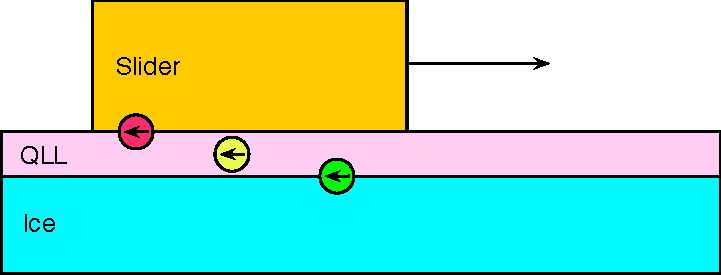
\includegraphics[width=\linewidth]{Figures/QLLsketch}
\caption{\label{fig:QLLsketch} In the hydrodynamic regime, the
  friction felt by a slider on an ice surface is mediated by a
  quasi-liquid layer (QLL) that forms on the surface of the ice.
  There can be many contributions to this friction: capillary bridges
  between the slider and the QLL (red), viscous drag in the liquid
  (yellow), and solid / liquid friction between the ice and the liquid
  film (green). This study concerns the last of the three
  contributions, the drag contributed by the ice-liquid interface.}
\end{figure*}

Kietzig \textit{et al.} have outlined popular experimental techniques
used to investigate the coefficients of friction for a variety of
materials sliding on ice, as well as their sensitivity to temperature,
slider load, contact area, wettability and hydrophobicity of the
slider.\cite{Kietzig2010} Of particular interest, the friction
coefficients were found to increase with increasing slider
velocity. This was attributed to three physical processes; adhesion
forces between the slider's asperities and the ice surface, breaking
of capillary bridges between the slider and the ice surface, and the
viscous shearing of the ice melt across the ice surface. While teasing
apart the individual contributions has proven challenging,
Kietzig\cite{Kietzig2009} and Persson\cite{Persson2015,Tuononen2016}
have made significant progress. However, there is still very little
known about water shearing over ice surfaces. Open questions include:
how does the structure of the interface change during this process,
and what role does the presented crystal facet have in the observed
friction?

\vspace{0.6cm}
\begin{flushleft}
\textit{Atomic Force Microscopy of the Surface of Ice}
\end{flushleft}

To probe the plastic deformation of ice surfaces, Pittenger \textit{et
  al.} have performed atomic force microscopy (AFM) experiments where
they indented the surface with an AFM tip.\cite{Butt2000,
  Pittenger2001,Bluhm2000} They found yield strengths of 14 MPa at
-10.4\degree~C, and 20 MPa at -15.1\degree~C; both are smaller than
Young's modulus of bulk ice. This indicates that the ice surface
undergoes plastic deformation during the indentation process. Butt
\textit{et al.}  argued that the rate of pressurized melting due to
the presence of the tip controlled the tip penetration
speed.\cite{Butt2000} However, Pettinger \textit{et al.} pointed out
that the pressure due to the tip was not large enough to cause melting
of the surface.\cite{Pittenger2001} They concluded that their AFM
experiments probed the deformation of an ice surface with the presence
of a QLL. Given that, the penetration rate of the AFM tip should be
governed by the rate of flow and viscosity of the QLL out from under
the tip. These AFM experiments indicate the viscosity of the surface
premelt must be at least 2 orders of magnitude greater than that of
bulk supercooled water. Li and Somorjai conjectured that the increase
in viscosity could be due to the confinement of the QLL between the
AFM tip and the ice, or due to the intrinsic ordering of the QLL
itself.\cite{Li2007}

Using lateral force microscopy (LFM), Bluhm \textit{et al.} have
obtained friction coefficients for ice grown on a mica substrate over
a temperature range of -40\degree~ to -24\degree~ C.\cite{Bluhm2000}
Plotting the lateral force against the imposed load, they were able to
extract a friction coefficient of about 0.6, which was robust over the
entire temperature range spanned. Since these results were comparable
to static friction coefficients observed in macroscopic measurements,
they conjectured that the QLL was pushed out from under the tip,
resulting in the tip having direct contact with the ice surface. 

Interpretation of AFM and LFM measurements of ice friction depends
strongly on whether a surface premelt layer is present between the tip
and the surface. However, since the viscosity of the quasi-liquid
layer is not known, nor how the fluid behaves confinement under the
tip, many of the reported results are open to conjecture.









% end iceWaterFriction intro


\section{Summary}
We began this chapter with an overview of molecular dynamics
simulations, including a brief discussion of water models and methods
to compute transport properties. Following this, we discussed
fundamental knowledge of ice, water, and characteristics of the
surface premelt. Lastly, we summarized our current
understanding of ice friction, arriving at open questions about the
effect the presented surface has on the premelt, and the
viscosity of the quasi-liquid layer.

In the chapters to follow, I present my contribution to our
understanding of friction at the surface of ice. In Chapter
\ref{chap:Methods} I describe the computational details and
methodologies used in simulating shearing at ice-I$_\mathrm{h}$ /
water interfaces. In Chapters \ref{chap:Str} and \ref{chap:Dyn}, I
investigate the structure and dynamics of the liquid at the interface,
and present estimates of the interfacial width. In Chapter
\ref{chap:Friction}, I present an appropriate friction coefficient for
no-slip boundary conditions, and explore possible mechanisms for the
observed facet dependent friction. In Chapter \ref{chap:QLL}, I
investigate the shear viscosity of the quasi-liquid layer, and compare
again supercooled liquid water. In Chapter \ref{chap:Concl}, I
summarize my work and conclude with projections of future
investigations.
